\newcommand{\clusteval}{\textbf{clusteval} }

\documentclass[12pt]{article}
\usepackage[latin1]{inputenc}
\usepackage[margin=3cm]{geometry}
\usepackage{graphicx}
\usepackage{multirow}
\usepackage{enumitem}
\usepackage[colorlinks=true,linkcolor=blue]{hyperref}
\usepackage{xcolor}
\usepackage{moreverb}
\usepackage{varwidth}
\usepackage{listings}

\lstset{prebreak=\raisebox{0ex}[0ex][0ex]
        {\ensuremath{\hookleftarrow}}}
\lstset{postbreak=\raisebox{0ex}[0ex][0ex]
        {\ensuremath{\hookrightarrow\space}}}
\lstset{breaklines=true}
\lstset{numbers=left}
\lstset{basicstyle=\ttfamily, numberstyle=\small\ttfamily}

\let\verbatiminput=\verbatimtabinput
\title{Technical Documentation: \clusteval
\\
\large An Integrated Clustering Evaluation Framework for Cluster Analysis}
\author{Christian Wiwie}
\date{\today}

\definecolor{gray}{rgb}{0.95,0.95,0.95}
%\renewcommand*{\labelitemi}{$\vdash$}
%\renewcommand*{\labelitemii}{$\vdash$}
%\renewcommand*{\labelitemiii}{$\vdash$}
%\renewcommand*{\labelitemiv}{$\vdash$}
\newcommand{\highlight}[1]{{\colorbox{gray}{\begin{varwidth}[b]{\dimexpr\linewidth-2\fboxsep}#1\end{varwidth}}}}
%\newcommand{\highlight}[1]{{\colorbox{gray}{#1}}}
%\newcommand{\highlight}[1]{#1}
\newcommand{\code}[1]{\texttt{\highlight{#1}}}
\newcommand{\codei}[1]{\texttt{\highlight{> #1}}}

\newcommand{\backendserver}{clustevalBackendServer.jar}
\newcommand{\backendclient}{clustevalBackendClient.jar}

\newcommand{\domain}{http://clusteval.mmci.uni-saarland.de}
\newcommand{\urltecdoc}{\domain/tecdoc.pdf}
\newcommand{\urlfrontend}{\domain/clustevalFrontend.zip}
\newcommand{\urlserver}{\domain/\backendserver}
\newcommand{\urlclient}{\domain/\backendclient}
\newcommand{\urlsources}{\domain/clustevalSources.zip}
\newcommand{\urljavadocs}{\domain/clustevalJavadocs.zip}
\newcommand{\vboxImage}{\domain/clustevalVbox.zip}

\newcommand{\vboxFrontend}{http://localhost/}
\newcommand{\vboxServer}{/home/clusteval/clustevalBackendServer.jar}
\newcommand{\vboxClient}{/home/clusteval/clustevalBackendClient.jar}

\newcommand{\repoconfigsuffix}{configs}
\newcommand{\repobasepath}{$<$REPOSITORY\_ROOT$>$}
\newcommand{\repodata}{\repobasepath/data}
\newcommand{\repodataconfigs}{\repodata/\repoconfigsuffix}
\newcommand{\repodatasets}{\repodata/datasets}
\newcommand{\repodatasetdir}{\repodatasets/$<$datasetFolder$>$}
\newcommand{\repodatasetfile}{\repodatasetdir/$<$datasetFile$>$}
\newcommand{\repodatasetconfigs}{\repodatasets/\repoconfigsuffix}
\newcommand{\repogoldstandards}{\repodata/goldstandards}
\newcommand{\repogoldstandarddir}{\repogoldstandards/$<$goldstandardFolder$>$}
\newcommand{\repogoldstandardfile}{\repogoldstandarddir/$<$goldstandardFile$>$}
\newcommand{\repogoldstandardconfigs}{\repogoldstandards/\repoconfigsuffix}
\newcommand{\repoprograms}{\repobasepath/programs}
\newcommand{\repoprogramconfigs}{\repoprograms/\repoconfigsuffix}
\newcommand{\repoprogramdir}{\repoprograms/$<$programFolder$>$}
\newcommand{\repoprogramexec}{\repoprogramdir/$<$executable$>$}
\newcommand{\reporprograms}{\repoprograms/$<$jarFile$>$}
\newcommand{\reporesults}{\repobasepath/results}
\newcommand{\reporesult}{\reporesults/$<$runIdentifier$>$}
\newcommand{\reporesultconfigs}{\reporesult/configs}
\newcommand{\reporesultgs}{\reporesult/goldstandards}
\newcommand{\reporesultinputs}{\reporesult/inputs}
\newcommand{\reporesultlogs}{\reporesult/logs}
\newcommand{\reporesultcluster}{\reporesult/clusters}
\newcommand{\reporesultanalyses}{\reporesult/analyses}
\newcommand{\reporuns}{\repobasepath/runs}
\newcommand{\reposupp}{\repobasepath/supp}
\newcommand{\reposuppclust}{\reposupp/clustering}
\newcommand{\reposuppparamopts}{\reposuppclust/paramOptimization}
\newcommand{\reposuppqualmeasures}{\reposuppclust/qualityMeasures}
\newcommand{\reposuppdistmeasures}{\reposupp/distanceMeasures}
\newcommand{\reposuppformats}{\reposupp/formats}
\newcommand{\reposuppinputformats}{\reposuppformats/dataset}
\newcommand{\reposuppresultformats}{\reposuppformats/runresult}
\newcommand{\reposuppgens}{\reposupp/generators}
\newcommand{\reposuppdsgens}{\reposuppgens/dataset}
\newcommand{\reposuppstats}{\reposupp/statistics}
\newcommand{\reposuppdatastats}{\reposuppstats/data}
\newcommand{\reposupprunstats}{\reposuppstats/run}
\newcommand{\reposupprundatastats}{\reposuppstats/rundata}
\newcommand{\reposupptypes}{\reposupp/types}
\newcommand{\reposuppdstypes}{\reposupptypes/dataset}

\begin{document}
	\maketitle
	\tableofcontents
	
	\newpage	
		\section{Introduction}\label{sec_intro}
	In the next chapter we will discuss briefly how \clusteval is organized, how it works in principle and what can be achieved through its use.
	
	Chapter \ref{sec_inst} explains, how the framework is to be installed and, amongst other things, what prerequisites are necessary to install and use it successfully. For Debian 6 (Squeeze) we provide a detailed step-by-step installation manual. For those of you, who do not want to install it manually but want to try out the framework right away, we offer a VirtualBox hard drive image which contains a Debian 6 installation, together with the framework and all its prerequisites (see \ref{subsec_vbox_image}).
	
	Chapter \ref{sec_usage} demonstrates the usage of the framework by a simple use case scenario from the very start to the very end. If you want more detailed information about the use cases \clusteval assists with, please  consult \cite{wiwie_2013}.
	
	If you are a programmer and you want to extend \clusteval, you will find more information in section \ref{sec_extend}.
	
	
	\section{The Framework}
	Our framework \clusteval is intended to perform automatized cluster analysis of arbitrary datasets and clustering methods. The goal is, that any clustering method known to the framework can be applied to any known dataset (with certain exceptions, partly inflicted by the clustering methods itself and partly inflicted by the framework constraints).
	
	In general \clusteval is divided into a backend and a frontend. Figure \ref{fig_general_structure} shows the general structure of the framework. The backend is reponsible for doing all the calculations including clusterings and the frontend has only visualization purposes.

\begin{figure}[hbtp]
\caption{General framework flow}
\label{fig_general_structure}
\centering
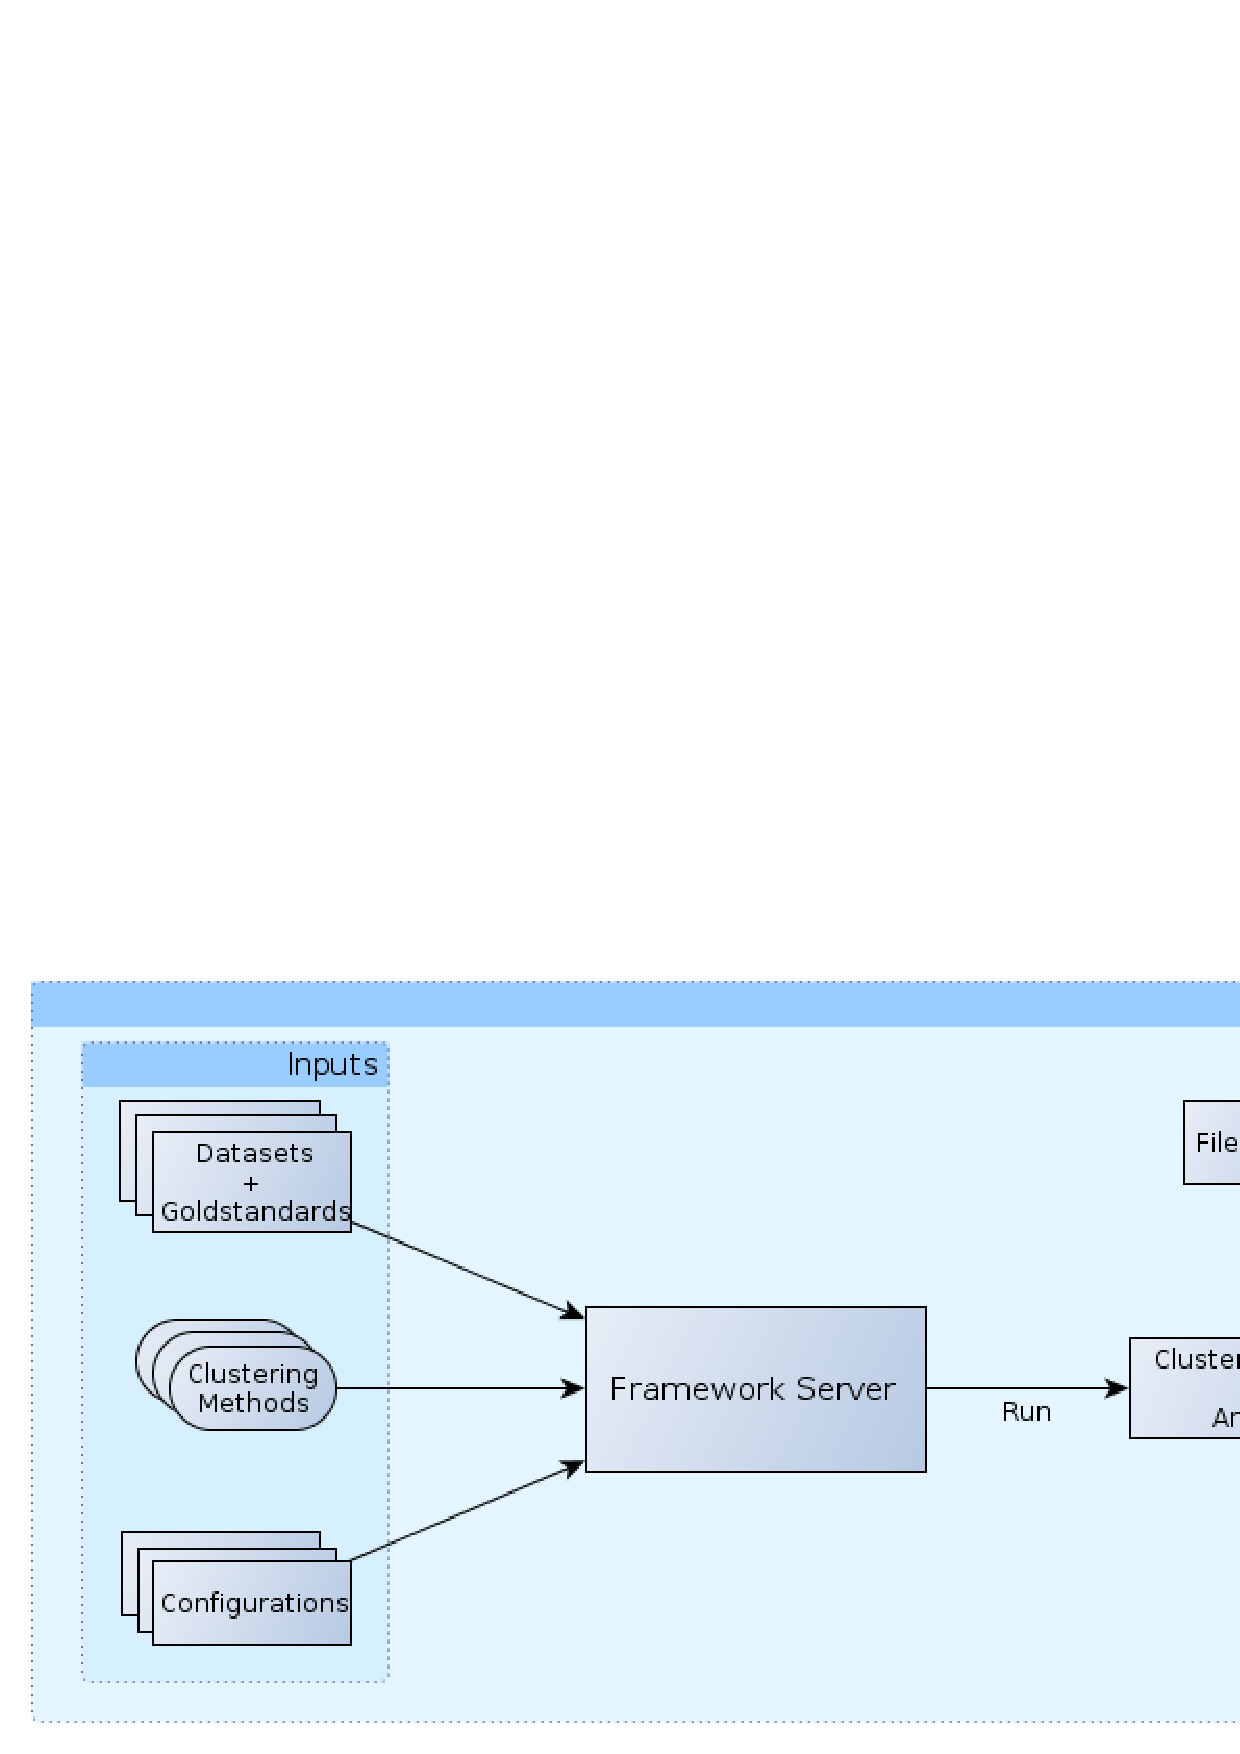
\includegraphics[width=\textwidth]{../master_seminar_presentation/framework_flow.png}
\end{figure} 

At first we will give an overview of the backend in \ref{subsec_general_backend} and then of the frontend in \ref{subsec_general_frontend}.

	
	\section{Backend}
	The backend of the framework is responsible for all calculations. It consists of a server and a client component. The server takes commands from the client and does the calculations internally and in a multithreaded way. The client can query the server to get the current status of a calculation or to give commands to the server which might control current processes. Figure \ref{fig_backend} shows the general structure of the backend and the components it contains.
	
\begin{figure}[hbtp]
\caption{The backend structure}
\label{fig_backend}
\centering
\includegraphics[width=\linewidth]{../master_seminar_presentation/framework_backend.png}
\end{figure}
	
	
	\section{Backend Server}\label{subsec_general_backend}
	 In principle the core of all tasks of the backend server is, to apply clustering methods to data (dataset and goldstandard) in an automatized and autonomous way, using only the configurations and inputs the user specified. The produced results have to be parsed in such a way, that the frontend can easily collect certain information and visualize them. Thus the components used by the backend that are not directly included into the framework programatically but need to be provided can be summarized as
	 \begin{itemize}
	 	\item Data (Datasets \& Goldstandards)
	 	\item Clustering Methods
	 	\item Configurations
	 \end{itemize}
	 
	 Additional components that can be extended and might be needed in case the provided standard functionality of the framework is not sufficient for the user

	\begin{itemize}
		\item Data input formats (including parsers)
		\item Run result formats (including parsers)
		\item Clustering Quality Measures
		\item Distance Measures
		\item Parameter Optimization Methods
		\item Dataset types
		\item (Data, Run \& Run-Data) Statistics
		\item Dataset generators
\end{itemize}		 
	 
	 All these components have to be located in the \textbf{repository} of the framework (see \ref{subsec_repository} for more details). The repository is a file system hierarchy located at a specified path and contains all components used by and available to the framework. Datasets, clustering methods or configurations outside the repository cannot be used by the framework.
	 
	 After these components have been made available to the backend, they can be combined almost arbitrarily. In the following we will describe the dependencies of each of these components which need to be fulfilled such that a new component of each type can be recognized and used by the framework.
	 

	\subsection{Repository}\label{subsec_repository}
		The backend server is based on a central repository which concludes all files in its folder structure. You can easily start a framework with a different set of files by simply using another repository.
		
		\begin{figure}[hbtp]
		\caption{Repository folder structure}
		\centering
		\includegraphics[width=\textwidth]{../master_seminar_presentation/repository_structure.png}
		\end{figure}
		

		\subsubsection{Repository folder structure}
			\begin{itemize}[noitemsep]
				\item \textbf{data}: Contains all data-related files.
				\begin{itemize}[noitemsep,nolistsep]
					\item \textbf{configs} [*.dataconfig]: Contains the data configuration files \ref{subsec:dataconfigs}.
					\item \textbf{datasets}: Contains all dataset-related files \ref{subsec:datasets}.
					\begin{itemize}[noitemsep,nolistsep]
						\item \textbf{configs} [*.dsconfig]: Contains the dataset configuration files \ref{subsubsec:datasetconfigs}.
						\item \textbf{[subfolder for every dataset]}: The dataset files themselves.
					\end{itemize}
					\item \textbf{goldstandards}: Contains all goldstandard-related files \ref{subsec:goldstandards}.
					\begin{itemize}[noitemsep,nolistsep]		
						\item \textbf{configs} [*.gsconfig]: Contains the goldstandard configurations \ref{subsubsec:gsconfigs}.
						\item \textbf{[subfolder for every goldstandard]}: Contains the goldstandard files themselves.
					\end{itemize}
				\end{itemize}
				\item \textbf{programs}: Contains all program-related files \ref{programs}.
				\begin{itemize}[noitemsep,nolistsep]
					\item \textbf{configs} [*.config]: Contains all program configuration files \ref{subsec_programconfigs}.
					\item \textbf{[subfolder for every program]}: The program files themselves.
				\end{itemize}
				\item \textbf{results}: The results of run executions \ref{runresults}.
				\begin{itemize}[noitemsep,nolistsep]
					\item \textbf{[subfolder for every run execution]}: A subfolder contains the results of one run execution.
					\begin{itemize}[noitemsep,nolistsep]
						\item \textbf{clusters}: The clustering results, including clustering qualities and graphics.
						\item \textbf{configs}: Copies of all used configuration files of this run execution to enable exact reproduction.
						\item \textbf{inputs}: Copies of all used inputs of this run execution to enable exact reproduction.
						\item \textbf{logs}: All log files corresponding to this run execution.
					\end{itemize}
				\end{itemize}
				\item \textbf{runs}: All run-related files \ref{sec:runs}.
				\begin{itemize}[noitemsep,nolistsep]
					\item \textbf{[*.run: a file for every run]}: Contains the run-files.
				\end{itemize}
				\item \textbf{supp}: Contains supplementary material.
				\begin{itemize}[noitemsep,nolistsep]
					\item \textbf{clustering}: Supplementary material related to clusterings.
					\begin{itemize}[noitemsep,nolistsep]
						\item \textbf{paramOptimization}: Contains clustering parameter optimization methods \ref{paramOptMethods}.
						\begin{itemize}[noitemsep,nolistsep]
							\item \textbf{[*.jar]}: Each jar-file corresponds to a parameter optimization method and is loaded dynamically by the framework.
						\end{itemize}
						\item \textbf{qualityMeasures}: Contains clustering quality measures \ref{clustQualMeasures}.
						\begin{itemize}[noitemsep,nolistsep]
							\item \textbf{[*.jar]}: Each jar-file corresponds to a clustering quality measure and is loaded dynamically by the framework.
						\end{itemize}
					\end{itemize}
					\item \textbf{formats}: Contains all formats used by the framework.
					\begin{itemize}[noitemsep,nolistsep]
						\item \textbf{dataset}: Contains all dataset formats \ref{formats}.
						\begin{itemize}[noitemsep,nolistsep]
							\item \textbf{[*.jar]}: Each jar-file corresponds to a dataset format and is loaded dynamically by the framework.
						\end{itemize}
						\item \textbf{runresult}: Contains all runresult formats \ref{formats}.
						\begin{itemize}[noitemsep,nolistsep]
							\item \textbf{[*.jar]}: Each jar-file corresponds to a runresult format and is loaded dynamically by the framework.
						\end{itemize}
					\end{itemize}
				\end{itemize}
			\end{itemize}
	 
	 \subsection{Clustering Methods}\label{programs}
	 Clustering Methods (technically also called \textbf{Programs} throughout this guide) can be executed by the framework, and be applied to data to calculate clusterings.
	 In order to include a new clustering method and use it within the framework, 
	\begin{itemize}		
		\item the \textbf{executable} of the method has to be made available to the framework (an exception are Clustering Methods provided through the R framework, see \ref{rprograms}), 
		\item the method itself has to be specified in a configuration file (called \textbf{program configuration})
		\item all other components (e.g. \textbf{input} and \textbf{output formats}) specified in the program configuration need to be available.
\end{itemize}
The configuration file for a clustering method (short \textbf{program configuration}) contains all information required, such that the framework can execute the method in an automatized and autonomous way. These information include for example, among others, the name of the method, its supported input formats, its output format, its parameters (including type and valid range of values). An exact description of how program configurations look like and which options and settings need to be specified can be found in \ref{subsec_programconfigs}.
	
	\clusteval ships with a set of clustering methods including
	\begin{itemize}
		\item Affinity Propagation
		\item Hierarchical Clustering$^{(Rserve)}$
		\item K-Means$^{(Rserve)}$
		\item Markov Clustering
		\item Spectral Clustering$^{(Rserve)}$
		\item Transitivity Clustering
	\end{itemize}
	
	For every of these clustering methods a \textbf{program configuration} is also provided, such that they are directly usable from the start. Of course these program configurations can be modified and adapted to the user's needs.
	
	\subsubsection{Standalone Programs}
	are programs that come as an executable. Those can be performed by the framework, after they have been specified in a program configuration. The executable needs to be compatible to the server architecture \clusteval runs on and they need to be executable (+x modifier). How you can add your own standalone programs into the framework can be found here \ref{subsubsec_extend_standprograms}
	\subsubsection{R Programs$^{(Rserve)}$}\label{rprograms} are programs, that are implemented within some R package. Arbitrary methods implemented in R can be used as a program, as long as they can be made available within R on the server. This implies that the corresponding R Program is available for your R version and that it can be compiled and installed on your server architecture. How you can add your own R Programs into the framework can be found here \ref{subsubsec_extend_rprograms}.
	
	\subsection{Datasets}\label{subsec:datasets}
	To add a dataset to the framework and make it usable, such that clustering methods can be applied to it, you have to
	\begin{itemize}		
		\item insert the dataset file into the repository of the backend
		\item insert a header into the dataset which specifies its format, format version and type
		\item specify the dataset in a configuration file (called \textbf{dataset configuration})
\end{itemize}
The dataset configuration contains the name and path of the dataset and other details how a possible conversion of the dataset should be handled. An exact description of how dataset configurations look like and which options and settings need to be specified can be found in \ref{subsubsec:datasetconfigs}.

\clusteval ships with a set of datasets of different types (PPI, Gene Expression, Protein similarity, Word-Sense disambiguation), for example 
	\begin{itemize}
		\item subsets of SCOP Astral95 v1.61,
		\item Brown et al. protein simliarities,
		\item leukemia microarray gene expression (Broad Institute),
		\item word context counts for word-sense disambiguation
	\end{itemize}
	
	\subsection{Goldstandards}\label{subsec:goldstandards}
	When assessing the qualities of a resulting clustering for most measures a goldstandard corresponding to the dataset is needed. The comparison of the clustering and goldstandard is then integrated into the calculation of the clustering quality measure (see \ref{clustQualMeasures}).
	
	Goldstandards for a dataset are \textbf{in principle optional}. Some operations can be also performed without a goldstandard and also some clustering quality measures do not require a goldstandard (for example Silhouette Value).
	
	Nevertheless, to be able to perform \textbf{all operations} on the dataset, a \textbf{goldstandard is required}.
	
	To add a goldstandard to the framework, you have to
	\begin{itemize}
		\item insert the goldstandard file into the repository of the backend
		\item specify the goldstandard in a configuration file (called \textbf{goldstandard configuration})
	\end{itemize}
	The goldstandard configuration contains the name and path to the goldstandard file. Since the framework does only support one goldstandard format, this does not need to be provided. An exact description of how goldstandard configurations look like and which options and settings need to be specified can be found in \ref{subsubsec:gsconfigs}.
	
	\subsection{Input \& Output formats}\label{formats}
	As already mentioned, datasets have their own formats and clustering methods can require different input and output formats. The general process how these formats link together can be visualized as seen in figure \ref{fig_format_conversion_processes}. 
	
	A dataset of a certain format known to the framework is converted into the standard input format of the framework using the parser belonging to the format of the dataset. Then the dataset in the standard format is converted to any of the supported input formats of the clustering method using the parser belonging to the chosen supported input format of the clustering method. Now the clustering method is applied to the dataset in the supported format. A clustering result is produced in the format of the clustering method. This result is then converted to the standard output format of the framework using the parser belonging to the format of the result. The framework then has access to the clustering results of the clustering method applied to the dataset in a format it understands, such that diverse operations can be performed on the result.
	
	\begin{figure}[hbtp]
	\caption{Format conversion processes}
	\label{fig_format_conversion_processes}
	\centering
	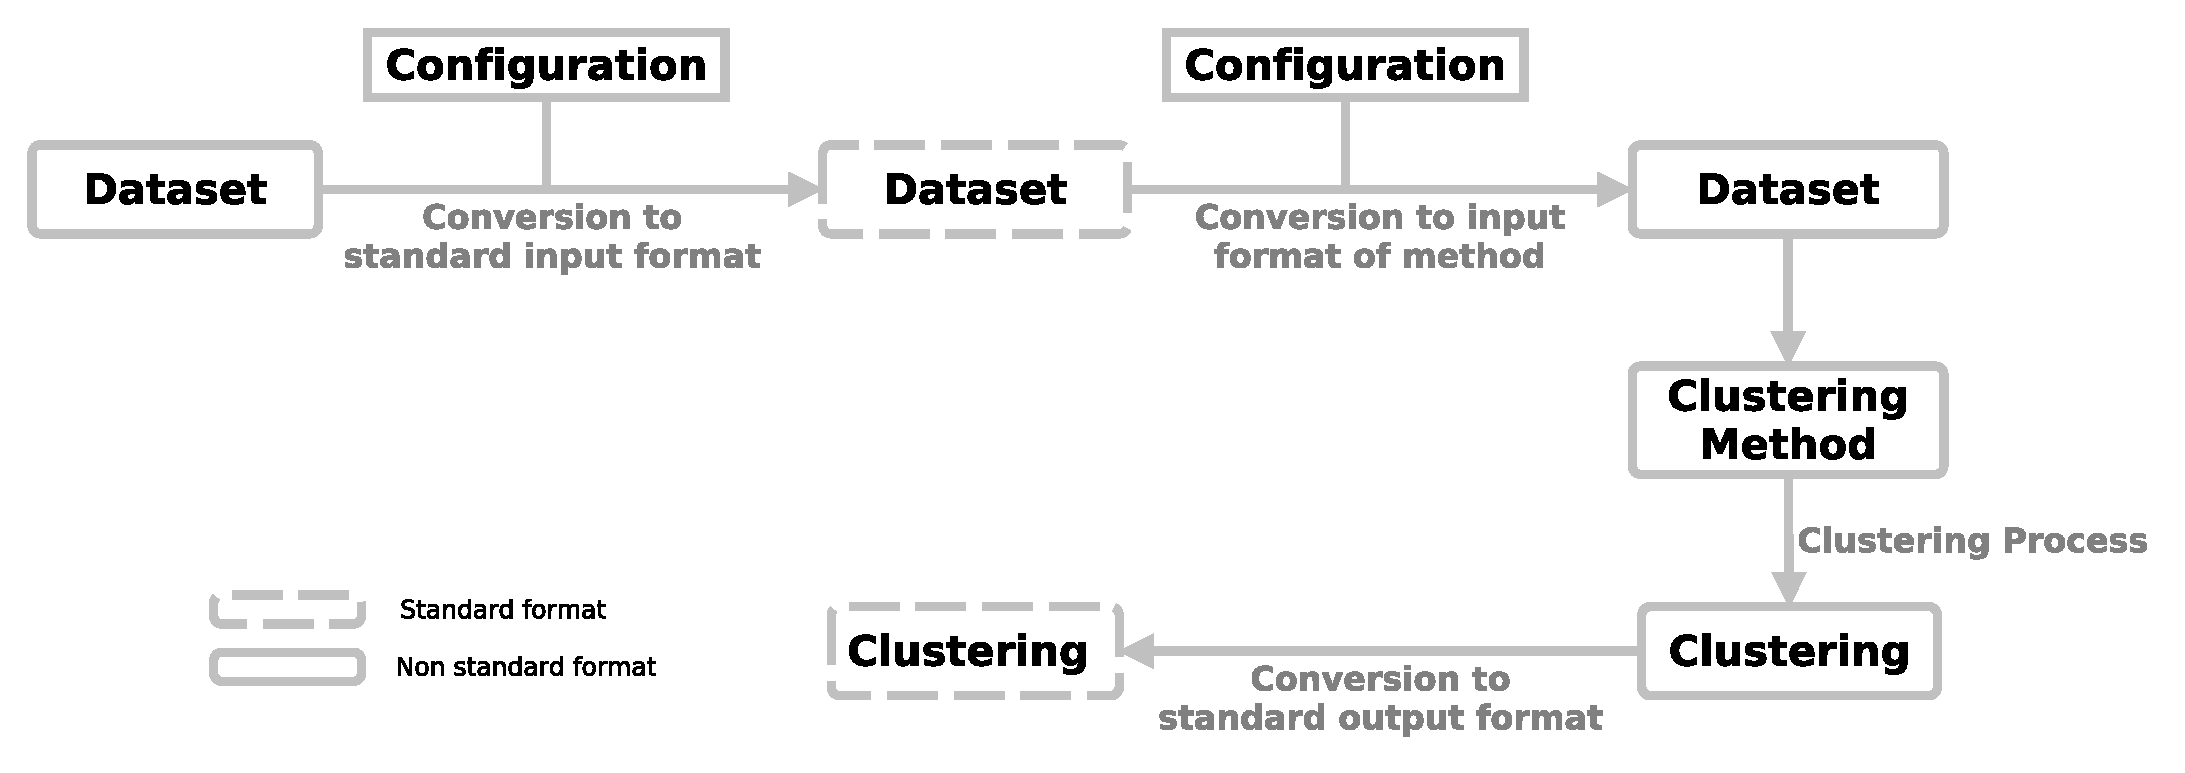
\includegraphics[width=.75\textwidth]{../master_seminar_presentation/flow_dataset.png} 
	\end{figure}

	If a new clustering method is added to the framework, its input and output formats need to be known to the framework. 
	
	\clusteval ships with a set of supported input and output formats. The input formats are
	
	\begin{itemize}
		\item APRowSimDataSetFormat
		\item BLASTDataSetFormat
		\item MatrixDataSetFormat
		\item RowSimDataSetFormat
		\item SimMatrixDataSetFormat
		\item TransClustSimMatrixDataSetFormat
	\end{itemize}
	and the output formats are
	\begin{itemize}
		\item APRunResultFormat
		\item MCLRunResultFormat
		\item TabSeparatedRunResultFormat
		\item TransClustRunResultFormat
	\end{itemize}
	
	If the new clustering method requires another input format not in the list, you will have to make it available to the framework by writing
	\begin{itemize}
		\item a wrapper class for this dataset format and 
		\item a parser, which converts the standardized input format of this framework to this input format.
	\end{itemize}
	If the new clustering method has a so far unknown output format, you will have to provide
	\begin{itemize}
		\item a wrapper class for this output format as well as
		\item a parser that converts that format to the standardized output format.
	\end{itemize}
	When this clustering method is applied to a dataset, the resulting clustering in the new format is converted to a standardized output format using your parser, such that further analyses can be performed regardless of the used clustering method.

For more information on how the framework can be extended by new input or output formats see \ref{formats} respectively.


	
			\subsubsection{Standard input format} \label{subsubsec:standarddatasetformat}
			The standard input format is a SimMatrixDataSetFormat which is described under \ref{subsubsec:simmatrixdatasetformat}.
			\subsubsection{APRowSimDataSetFormat}\label{aprowsimdatasetformat}
				This input format is used by Affinity Propagation. It is similar to the RowSimDataSetFormat, except that it accepts only numbers as ids and that it leaves out lines where id1=id2 such that it looks like this:
				\begin{lstlisting}
1	2	0.2
1	3	0.6
2	1	0.2
2	3	0.5
3	1	0.6
3	2	0.5				\end{lstlisting}
			\subsubsection{BLASTDataSetFormat}
				The BLAST dataset format needs a all-vs-all BLAST file and a corresponding FASTA file.
				
				\textbf{Please note}, that the FASTA file has to be named exactly like the BLAST file plus the additional .fasta extension. If the BLAST file is named like MyBlastFile.blast, then the FASTA file only be found by the framework, when it lies in the same directory and is named MyBlastFile.blast.fasta.
				
			\begin{lstlisting}
d1dlwa_	d1dlwa_	77.59	116	0	0	1	116	1	116	4.4e-46	172.6
d1dlwa_	d1idra_	40.30	67	40	0	19	85	31	97	3.2e-12	60.08
d1dlwa_	d1dlya_	32.00	100	62	1	19	116	19	118	1.6e-11	57.77
d1dlwa_	d2gdm__	45.45	22	12	0	60	81	89	110	0.435	23.10
d1dlwa_	d1cqxa1	37.50	24	15	0	62	85	79	102	0.969	21.94
d1dlwa_	d1cqxa1	40.00	5	3	0	71	75	134	138	4975.0	9.62
d1dlwa_	d1kr7a_	31.25	32	22	0	41	72	45	76	  4.8	19.63
d1dlwa_	d1kr7a_	50.00	8	4	0	50	57	91	98	202.0	14.24
d1dlwa_	d1kr7a_	66.67	3	1	0	50	52	86	88	6497.5	9.23
d1dlwa_	d1edg__	45.00	20	11	0	47	66	262	281	  6.3	19.25			\end{lstlisting}
				
			\begin{lstlisting}
>d1dlwa_
slfeqlggqaavqavtaqfyaniqadatvatffngidmpnqtnktaaflc
>d1dlya_
slfaklggreaveaavdkfynkivadptvstyfsntdmkvqrskqfafla
>d1idra_
gllsrlrkrepisiydkiggheaievvvedfyvrvladdqlsaffsgtnm
>d1kr7a_
mvnwaavvddfyqelfkahpeyqnkfgfkgvalgslkgnaayktqagktv\end{lstlisting}

			\subsubsection{MatrixDataSetFormat}
			This input format is a absolute dataset format, that means it contains samples together with their absolute coordinates:
			
\begin{lstlisting}
ALL_19769_B.cell	759	169	54	36
ALL_19769_B.cell_2	1062	88	235	38
ALL_28373_B.cell	822	196	150	120
ALL_28373_B.cell_2	1068	146	221	16
ALL_9692_B.cell		1455	53	217	169
\end{lstlisting}
			 

			\subsubsection{RowSimDataSetFormat}
				This input format consists of tab-separated rows looking as follows:
				\begin{lstlisting}
id1	id1	1.0
id1	id2	0.2
id1	id3	0.6
id2	id1	0.2
id2	id2	1.0
id2	id3	0.5
id3	id1	0.6
id3	id2	0.5
id3	id3	1.0				\end{lstlisting}
				
			\subsubsection{SimMatrixDataSetFormat} \label{subsubsec:simmatrixdatasetformat}
			 The SimMatrixDataSetFormat is a complete quadratic tab-separated similarity matrix with header row and column (containing ids). A dataset file with the SimMatrixDataSetFormat could look as follows:
			\begin{lstlisting}
	id1	id2	id3
id1	1.0	0.2	0.6
id2	0.2	1.0	0.5
id3	0.6	0.5	1.0
\end{lstlisting}
			There are no spaces in this file, only tabs. It does not necessarily need to be symmetric, it depends on the clustering method, whether it supports asymmetric similarity data.
			
			\subsubsection{TransClustSimMatrixDataSetFormat}
			This format can be used by Transitivity Clustering and it looks as follows:
			\begin{lstlisting}
3	
id1
id2
id3
0.2	0.6
0.5
\end{lstlisting}

	The number in the first line is the number of ids. It is followed by all ids in the next lines. Then it follows the tab-separated upper half of the similarity matrix. This format expects that the similarity matrix is symmetric.
	

		\subsubsection{Standard output format} \label{subsubsec:standardrunresultformat}
		The standard output format contains one clustering generated for parameter values $p_1=v1$,...,$p_K=vK$ in one line with clusters $c1,...,cK$, cluster sizes $size(ci) = si$. Every cluster $ci$ contains elements $e\_i\_1,...,e\_i\_si$ with fuzzy coefficients $f\_i\_1,...,f\_i\_si$. The format for this looks as follows:
		
		\begin{verbatim}
p1,...,pK	Clustering
v1,...,vK	e_1_1:f_1_1,...,e_1_s1:f_1_s1;...;e_K_1:f_K_1,...,e_K_sK:f_K_sK
	\end{verbatim}
	
	The parameter names and values on the left have to be separated by a TAB from the string "Clustering" and the clustering on the right. If the fuzzy coefficients are missing, the framework will not be able to parse the result file.
		
		\subsubsection{APRunResultFormat}
		This is the result format of Affinity Propagation.
		\subsubsection{MCLRunResultFormat}
		This is the result format of Markov Clustering.
		\subsubsection{TransClustRunResultFormat}
		This is the result format of Transitivity Clustering.
		

	\subsection{Clustering Quality Measures}\label{clustQualMeasures}
	The clustering quality measures are used by the framework to assess the quality of calculated clusterings. \clusteval ships with a standard set of clustering quality measures
	\begin{itemize}
		\item F1 \& F2-Score
		\item False Discovery Rate (FDR)
		\item False Positive Rate (FPR)
		\item Rand Index
		\item Sensitivity
		\item Specificity
		\item Silhouette Value (Java \& R implementation)
	\end{itemize}
	Please check \ref{clustQualMeasures} for more information on how to extend the framework by new clustering quality measures.
	\subsection{Distance Measures}\label{distanceMeasures}
	 The distance measures are used when converting absolute datasets (containing absolute coordinates) to relative datasets (pairwise similarities). The distance measures define how to assess the similarity between a pair of objects given their absolute coordinates.
	\clusteval ships with the following distance measures
	\begin{itemize}
		\item Euclidian
		\item Hoeffding D Statistic$^{(Rserve)}$
		\item Pearson Correlation Coefficient$^{(Rserve)}$
		\item Spearman Correlation Coefficient$^{(Rserve)}$
	\end{itemize}
	Please check \ref{distanceMeasures} for more information on how to extend the framework by new distance measures.
	\subsection{Parameter Optimization Methods}\label{paramOptMethods}
	 The backend can perform automatized and autonomous optimization of parameters of clustering methods. This is an iterative procedure where the backend assesses qualities of clustering results of the last iteration and adapts the parameter for the next iteration in order to find optimal parameters for the method on the given data. The parameter optimization method determines the following aspects:

\begin{enumerate}
\item the number of iterations of the optimization process
\item the parameter sets evaluated
\item the handling of diverging iterations
\item the storage of the iteration results in RAM
\end{enumerate}


	\clusteval ships with the following set of parameter optimization methods
	\begin{itemize}
		\item Affinity Propagation Divisive Parameter Optimization Method
		\item Affinity Propagation Parameter Optimization Method
		\item Divisive Parameter Optimization Method
		\item Gap Statistic Parameter Optimization Method
		\item Layered Divisive Parameter Optimization Method
		\item Transitivity Clustering Parameter Optimization Method
		\item Transitivity Clustering Quantile Parameter Optimization Method
	\end{itemize}
	Detailed information about each of these methods can be found in \cite{wiwie_2013}. Please check \ref{paramOptMethods} for more information on how to extend the framework by new parameter optimization methods.
	

	
	\subsection{Configuration Files}
	Above we already discussed that the framework needs \textbf{program configurations}, \textbf{dataset configurations} and \textbf{goldstandard configurations}. Those configuration files directly reference corresponding files (dataset, goldstandard, \ldots) on the filesystem. Internally the framework has some abstraction layers to store all the configurations. Figure \ref{fig_backend_configurations} shows the overall abstractional structure of the configuration files used in the backend. One can see that dataset- and goldstandard configuration are linked together in a \textbf{data configuration}.
	
	A run is an abstract entity that can be performed by the backend. Its execution involves (in most cases) application of clustering methods to several datasets, and afterwards clustering qualities are assessed using the goldstandards corresponding to each dataset. A run corresponds to a \textbf{run configuration} file, which then again references the \textbf{program-} and \textbf{data configurations} that should be pairwise combined.
	
	When a run is performed by the backend, the clustering methods wrapped by all referenced program configurations are applied to all datasets indirectly referenced through the data configurations.
	
	
	\begin{figure}[hbtp]
	\caption{Backend Configurations}
	\label{fig_backend_configurations}
	\centering
	\includegraphics[width=.75\textwidth]{../master_seminar_presentation/backend_configurations.png} 
	\end{figure}
	

	
		\subsubsection{Data Configurations} \label{subsec:dataconfigs}
		A data configuration is a file, that combines two other configurations together: A dataset configuration (see \ref{subsubsec:datasetconfigs}) and a goldstandard configuration (see \ref{subsubsec:gsconfigs}). Later on when you create a run (and its configuration) and in this run you want to apply two clustering methods to three datasets (together with their goldstandards) you will do so by telling the run configuration the names of the three corresponding data configurations. \textbf{Please note:} The data configuration file has to have the file extension .dataconfig, otherwise it will not be recognized by the framework.
		\begin{description}
		\item[datasetConfig:]
			This option has to be set to the name of the dataset configuration (see \ref{para:datasetName}), \textit{not} the name of the file.
			
		\item[goldstandardConfig:]
			This option has to be set to the name of the goldstandard configuration (see \ref{para:goldstandardName}), \textit{not} the name of the file.
		\end{description}
			
		\subsubsection{Example Data Configuration} A data configuration could like as follows:
\begin{listing}{1}
datasetConfig = astral_1
goldstandardConfig = astral_1_161\end{listing}


		
			\subsubsection{Dataset Configuration} \label{subsubsec:datasetconfigs}
			A dataset configuration tells the framework meta information about the corresponding dataset. That is: The internal name of the dataset, its filename and its format.
			
			\begin{description}
			\item[datasetName:] \label{para:datasetName}
			This name is used to find and access datasets within the framework. The name of the dataset \textit{has} to be identical to the subfolder of the corresponding dataset.
			\item[datasetFile:] \label{para:datasetFile}
			This option has to be set to the filename of the dataset file residing within the subfolder of the dataset.
			\item[datasetFormat:] \label{para:datasetFormat}
			This option tells the framework, which format the dataset is in. \clusteval ships with a set of supported dataset formats. Please note, that the entries in this list \textit{have} to be identical with the simple names of the corresponding dataset format classes.
			\item[[distanceMeasureAbsoluteToRelative:]] This indicates, which distance measure should be used, when this dataset is converted to another format. Defaults to EuclidianDistanceMeasure.
			\item[[preprocessorAfterDistance:]]A comma seperated list of data
				 preprocessors to apply, before the data is converted to pairwise
				 similarities (the standard input format)
			\item[[preprocessorAfterDistance:]] A comma seperated list of data
				 preprocessors to apply, after the data is converted to pairwise
				 similarities (the standard input format)
			\end{description}
	
			\subsubsection{Example Dataset Configuration}
			
			\begin{listing}{1}
datasetName = astral_1_161
datasetFile = blastResults.txt
datasetFormat = BLASTDataSetFormat
distanceMeasureAbsoluteToRelative = EuclidianDistanceMeasure \end{listing}

			\subsubsection{GoldStandard Configuration} \label{subsubsec:gsconfigs}
			A goldstandard configuration tells the framework meta information about the corresponding goldstandard. That is: The internal name of the goldstandard and its filename.
			
			\begin{description}
			\item[goldstandardName:] \label{para:goldstandardName}
			This name is used to find and access goldstandards within the framework. The name of the goldstandard \textit{has} to be identical to the subfolder of the corresponding goldstandard.
			\item[goldstandardFile:] \label{para:goldstandardFile}
			This option has to be set to the filename of the goldstandard file residing within the subfolder of the goldstandard.
			\end{description}
	
			\subsubsection{Example Goldstandard Configuration}
			
			\begin{listing}{1}
goldstandardName = astral_1_161
goldstandardFile = astral_161.goldstandard_3.txt \end{listing}
			
	

		\subsubsection{Program Configurations} \label{subsec_programconfigs}
		For every clustering method there can be several configuration files. All program configurations have to be located in \highlight{\repoprogramconfigs}. A program configuration tells the framework, what parameters the program expects, how to invoke the executable, with what parameter values to invoke it and several other information. Possible entries in a program configuration follow.
		
		\textbf{Please note:} The program configuration file has to have the file extension \highlight{.config}, otherwise it will not be recognized by the framework.
		
	\begin{description}
		\item[type:] Indicates, whether the program described by this program configuration is a standalone or an R program. This option can be set to either \textit{standalone} or the simple name of the R program class.

		\item[program:] This is the full name of the clustering method, this configuration references. When a clustering method is located in \highlight{\repoprograms/some/program}, then the full name of the program is "some/program"
		
		\item[alias:] This option is only interpreted for standalone programs. It tells the framework a alias of the corresponding program, which is used whenever the program needs to be represented in a readable format, e.g. on the website.
		
		\item[parameters:] 	A comma-separated list of parameters the program uses and which can be used when the program is invoked. These parameters need to be set to valid values before the program is actually applied to a dataset. Parameter values can be specificely defined either in a program or run configuration or, in case of parameter optimization runs, they are autonomously determined by the framework. If no value is defined for a program parameter at all, it will be set to its default value given in the program configuration.
		
		\item[optimizationParameters:] This option is only used, when a run is performed in parameter optimization mode. Then this list of parameters (that needs to be a subset of the list given in option "parameters") is used to determine, which parameters can be in principle optimized when this program is used in parameter optimization mode.
		
		\item[compatibleDataSetFormats:] This list tells the framework, which input formats this program supports. Please note, that the entries in this list \textit{have} to be identical to the simple names of the classes of the corresponding dataset formats.
		
		\item[outputFormat:] This option tells the framework, what the output format of this program is. Please note, that the naming convention of this list follows the same rules as those of "compatibleDataSetFormats", as the value of this option has to be named exactly after the simple name of the corresponding class.
		
		\item[expectsNormalizedDataSet:] This option can be set to "true" or "false". By default, it is set to false. If you set it to true, the input similarities (only) for this program are normalized to values between 0 and 1. This may help you, if a clustering method does not support negative values or values outside certain ranges.
		
		\item[[invocationFormat]] This is the section containing a set of invocation formats which tell the framework in string format, how to invoke this program. The invocation formats may contain program parameters or certain predefined variables, which are replaced by the framework during runtime. Such variable names are enclosed by \% signs. All program parameters defined in the parameters section of the program configuration can be used in the invocation format string. Additionally the following variables are hardcoded for every program and cannot be used for other parameters:
			\begin{description}
				\item[\%e\%] will be replaced by the absolute path of the executable
				\item[\%i\%] will be replaced by the absolute path of the input
				\item[\%o\%] will be replaced by the absolute path of the output
				\item[\%gs\%] will be replaced by the absolute path of the goldstandard
			\end{description}
			
			For example, if the option is set like this:
			
				\code{invocationFormat = \%e\% \%i\% \%preference\% \%o\% maxits=\%maxits\% convits=\%convits\%}
				
			"preference", "maxits" and "convits" have to be defined in the "parameters" entry of the same program configuration.
			
	\begin{description}
		\item[invocationFormat:]
			This is the option which tells the framework, how to invoke this program in case we have a goldstandard and no parameter optimization run. All words enclosed with \% will be replaced by the framework at runtime. All other variables in the invocation line have to be parameters defined in this program configuration.
			
		\item[invocationFormatWithoutGoldStandard:]
			This is how to invoke this program in case we have no goldstandard and no parameter optimization run.
			
		\item[invocationFormatParameterOptimization:]
			This is how to invoke this program in case we have a goldstandard and a parameter optimization run.
			
		\item[invocationFormatParameterOptimizationWithoutGoldStandard:]
			This is how to invoke this program in case we have no goldstandard and a parameter optimization run.
		\end{description}
		\item[[$<$parameterName$>$]]
			For every parameter defined in the list of entry "parameters", there needs to be an additional section in the program configuration, which tells the framework several information about the parameter:
			\begin{description}
				\item[desc:] A description of the parameter
				\item[type:] One of the types FLOAT ("2"), INTEGER ("1") or STRING ("0").
				\item[def:] A default value for the parameter.
				\item[minValue:] The minimal value for the parameter.
				\item[maxValue:] The maximal value for the parameter.
			\end{description}
	\end{description}
			
		\subsubsection{Example program configuration}
		%\fontsize{10pt}{12pt}
		\begin{listing}{1}
program = APcluster
parameters = preference,maxits,convits,dampfact
optimizationParameters = preference,maxits,convits,dampfact
executable = apcluster
compatibleDataSetFormats = APRowSimDataSetFormat
outputFormat = APRunResultFormat

[invocationFormat]
invocationFormat = %e %i %preference %o maxits=%maxits convits=%convits 
dampfact=%dampfact

[maxits]
desc = Max iterations
type = 1
def = 2000
minValue = 2000
maxValue = 5000

[convits]
desc = Cluster Center duration
type = 1
def = 200
minValue = 200
maxValue = 500

[dampfact]
type = 2
def = 0.9
minValue = 0.7
maxValue = 0.99

[preference]
desc = Preference
type = 2
def = 0.5
minValue = 0.0
maxValue = 1.0		\end{listing}


	
	\subsection{Runs} \label{sec:runs}

\begin{figure}[hbtp]
\caption{Inheritance of different run types}
\label{fig_run_inheritance}
\centering
\includegraphics[width=.6\textwidth]{../master_seminar_presentation/run_inheritance.png}
\end{figure} 
	
		Runs are entities that can be performed by the backend server. A run is defined by a file in the folder \highlight{\reporuns}. The name of that file (without extension) also defines the name of the run. Depending on the type of the run this file contains several other components which configure the process when the run is performed. Figure \ref{fig_run_inheritance} shows the different types of runs and how they relate to each other.
		
		\subsubsection{Run Files} \label{run_files}
		
		Every run is defined in a run-file in the corresponding folder of the repository. Depending on the type of the run, different options are available that can be specified in the run-file. Common to all types of runs are the following options:
		
		\begin{description}
			\item[mode:] \label{subsubsec:runconfigmode}
				This entry can be set to "clustering",  "parameter\_optimization", "dataAnalysis", "runAnalysis" or "runDataAnalysis". These types can be found in the aforementioned figure and are described in the following paragraphs.
		\end{description}
		
		\subsubsection{Execution Runs} \label{execution_runs}		
			Execution runs calculate clusterings during their execution and assess qualities for every of those clusterings. Clusterings are calculated by applying clustering methods to datasets using a certain parameter set. That is why execution runs have sets of both, program and data configurations. During execution time every program configuration is applied to every data configuration in a pairwise manner. For every calculated clustering a set of clustering quality measures are assessed.
			
		  In general the options of such a combination of data and program configuration will be taken from these configurations respectively, but can be overridden by the options in the run configuration, That means parameter values defined in the program as well as in the run configuration will be taken from the latter.
		 
		 \subsubsection{Execution Run Files}\label{execution_run_files} For execution runs, additionally to the options defined for all runs (see \nameref{run_files}), the following options for the run-file are defined:
		 \begin{description}
			\item[programConfig:]
			This entry has to be set to a single name or a comma-separated list of names of program configurations. When this run is performed, these program configurations will be pairwise combined with the data configurations given in the option "dataConfig". 
			\item[dataConfig:]
			This entry has to be set to a single name or a comma-separated list of names of data configurations. When this run is performed, these data configurations will be pairwise combined with the program configurations given in the option "programConfig". 
			\item[qualityMeasures:] \label{subsubsec:runconfigqualmeasure}
				This option determines, which quality measures will be assessed for every clustering calculated during the run process. When this run is a clustering run (see option "mode"), then for every pair of data and program configurations there will be only one clustering as a result for which quality measures will be evaluated. When the mode is set to "parameter\_optimization", for every iteration during the parameter optimization process these quality measures will be evaluated.
			\item[[$<$programConfigName$>$]:]
			If a dedicated section is found in this run file that is called like one of the program configurations given in option "programConfig", several parameters can be overridden individually only for this program configuration which are
			\begin{description}			 	
				\item[$<$parameterName$>$:] The program parameter with the given name which needs to be defined in the program configuration can be fixed to a certain value.
\end{description}
		 \end{description}
		  
		 \subsubsection{Clustering Runs}\label{clustering_runs}
		 Clustering runs are a type of execution run, that means they calculate clusterings by applying every program configuration to every data configuration. Afterwards they assess the qualities of those clusterings in terms of several clustering quality measures.
		 
		 In the case of clustering runs for every pair of program and data configuration exactly one clustering is calculated and assessed. Clustering runs are visualized in figure \ref{clustering_run_process}.
		 
		 \begin{figure}[hbtp]
		 \caption{Clustering Run Process}
		 \label{clustering_run_process}
		 \centering
		 \includegraphics[width=\linewidth]{../master_seminar_presentation/framework_flow_singleclustering.png}
		 \end{figure}
		 
		 \paragraph{Clustering Run File} For clustering runs, the options are the same as for all execution runs (see \nameref{execution_run_files}).
		 
		  
		 \subsubsection{Parameter Optimization Runs}\label{paramOpt_runs}
		 Parameter optimization runs are a type of execution run, that means they calculate clusterings by applying every program configuration to every data configuration. Afterwards they assess the qualities of those clusterings in terms of several clustering quality measures.
		 
		In contrast to clustering runs, parameter optimization runs calculate several clusterings for every pair of data and program configuration in a pairwise manner. Every clustering corresponds to a certain parameter set and the parameter sets to evaluate are determined by a parameter optimization method (see \ref{paramOptMethods} for more information). Parameter optimization runs are visualized in figure \ref{paramOpt_run_process}.
		
		\begin{figure}[hbtp]
		\caption{Parameter Optimization Run Process}
		\label{paramOpt_run_process}
		\centering
		\includegraphics[width=\linewidth]{../master_seminar_presentation/framework_flow_parameterOptimization.png}
		\end{figure}
		
		\paragraph{Parameter Optimization Run File}\label{paramOpt_run_files}
		
		For parameter optimization runs, additionally to the options defined for all execution runs (see \nameref{execution_run_files}), the following options for the run-file are defined:
		 \begin{description}
		 	\item[optimizationMethod:] The parameter optimization method to use when this run is performed.
		 	\item[optimizationCriterion:] The clustering quality measure which should be used as optimization criterion. This criterion is used to determine the optimal parameter set during the optimization process. Therefore it can influence the cause of the optimization process, if the chosen parameter optimization method integrates the qualities of previous iterations into future iterations.
		 	\item[optimizationIterations:] The number of total optimization iterations that should be performed for every pair of program and data configuration. \textbf{Hint:} This number might not be the number, the optimization process performs in the end, since it gives only a desirable number that might not be accurately realizable for a specific optimization method.
			\item[[$<$programConfigName$>$]:]
			If a dedicated section is found in this run file that is called like one of the program configurations given in option "programConfig", several parameters can be overridden individually only for this program configuration which are
			\begin{description}			 	
				\item[optimizationParameters:] A comma separated list of the parameters that should be optimized for this program configuration
				\item[optimizationMethod:] The parameter optimization method to use for this program configuration
\end{description}
		 \end{description}
		
		
		\subsubsection{Analysis Runs} \label{analysis_runs}		
			Analysis runs assess certain properties of objects of interest. An analysis run has a set of target objects and a set of statistics, that should be assessed for each of the target objects. That means, during execution time for every target object every statistic is assessed in a pairwise manner.
		
		\subsubsection{Data Analysis Runs} \label{dataAnalysis_runs}		
			In case of data analysis runs the target objects to analyze are data configurations (indirectly datasets) and the statistics are data statistics, that is properties of datasets. Data analysis runs are visualized in figure \ref{dataAnalysis_run_process}.
		
		\begin{figure}[hbtp]
		\caption{Data Analysis Run Process}
		\label{dataAnalysis_run_process}
		\centering
		\includegraphics[width=\linewidth]{../master_seminar_presentation/framework_flow_dataAnalysis.png}
		\end{figure}
		
		\subsubsection{Data Analysis Run File}\label{dataAnalysis_run_file}

		For data analysis runs the following options for the run-file are defined:
		 \begin{description}
		 	\item[dataStatistics:] A comma separated list of data statistics to assess for the given data configurations.
		 	\item[dataConfig:] A comma separated list of data configurations to analyse.
		 \end{description}
			
		
		\subsubsection{Run Analysis Runs} \label{runAnalysis_runs}		
			In case of run analysis runs the target objects to analyze are clusterings (results of execution runs) and the statistics are run statistics, that is properties of execution run results. Run analysis runs are visualized in figure \ref{runAnalysis_run_process}.
		
		\begin{figure}[hbtp]
		\caption{Run Analysis Run Process}
		\label{runAnalysis_run_process}
		\centering
		\includegraphics[width=\linewidth]{../master_seminar_presentation/framework_flow_runAnalysis.png}
		\end{figure}
		
		\subsubsection{Run Analysis Run File}\label{runAnalysis_run_file}

		For run analysis runs the following options for the run-file are defined:
		 \begin{description}
		 	\item[runStatistics:] A comma separated list of run statistics to assess for the given execution run results.
		 	\item[uniqeRunIdentifiers:] A comma separated list of identifiers of execution run results. See \ref{runresults} for an explanation on run result identifiers.
		 \end{description}
		
		\subsubsection{Run-Data Analysis Runs} \label{runDataAnalysis_runs}		
			In case of run-data analysis runs the target objects to analyze are pairs of data configurations and clusterings (results of execution runs) and the statistics are run-data statistics, that is relationships between execution run results and properties of data configurations. Run-Data analysis runs are visualized in figure \ref{runDataAnalysis_run_process}.
		
		\begin{figure}[hbtp]
		\caption{Run-Data Analysis Run Process}
		\label{runDataAnalysis_run_process}
		\centering
		\includegraphics[width=\linewidth]{../master_seminar_presentation/framework_flow_runDataAnalysis.png}
		\end{figure}
		
		\subsubsection{Run-Data Analysis Run File}\label{runDataAnalysis_run_file}

		For run-data analysis runs the following options for the run-file are defined:
		 \begin{description}
		 	\item[runDataStatistics:] A comma separated list of run-data statistics to assess for every pair of given execution run result and data analysis result.
		 	\item[uniqeRunIdentifiers:] A comma separated list of identifiers of execution run results. See \ref{runresults} for an explanation on run result identifiers.
		 	\item[uniqeDataIdentifiers:] A comma separated list of identifiers of data analysis run results. See \ref{runresults} for an explanation on run result identifiers.
		 \end{description}
			
			\subsubsection{Examples of a Run Configurations}
			
			See \ref{fig:runconfig1} and \ref{fig:runconfig2} for examples of run configuration files.
			
			\begin{figure}[hbtp]
			\label{fig:runconfig1}
			\caption{Example run configuration "all\_vs\_astral\_1\_171.runconfig" for Parameter Optimization Mode}
			\begin{lstlisting}
programConfig = APcluster_1,TransClust_2,MCL_1
dataConfig = astral_1_171
qualityMeasures = TransClustF2ClusteringQualityMeasure,SilhouetteValueRClusteringQualityMeasure
mode = parameter_optimization
optimizationMethod = DivisiveParameterOptimizationMethod
optimizationCriterion = SilhouetteValueRClusteringQualityMeasure
optimizationIterations = 1001

[TransClust_2]
optimizationParameters = T

[MCL_1]
optimizationParameters = I

[APcluster_1]
optimizationParameters = preference,dampfact,maxits,convits
optimizationMethod = APDivisiveParameterOptimizationMethod\end{lstlisting}
			\end{figure}
			
			\begin{figure}[hbtp]
			\label{fig:runconfig2}
			\caption{Example run configuration "mcl\_1.runconfig" for Clustering mode}
			\begin{lstlisting}
programConfig = MCL_1
dataConfig = DS1,test50

[MCL_1]
I = 2.0			\end{lstlisting}
			\end{figure}
			
	\subsection{Run Results}\label{runresults}

	When a run is performed, a unique run identifier is determined which includes the starttime and date and the name of the run. If the run \highlight{exampleRun} is performed at the 5th of July 2012 at 12:58:38, its unique run identifier is \highlight{06\_05\_2012-12\_58\_38\_exampleRun} which is also used as the subfolder to store its results in
	
	\highlight{\reporesults/06\_05\_2012-12\_58\_38\_exampleRun}
	
	Every such folder contains some subfolders. Common to all run types are the following subfolders:
	
	\subsubsection{All run result} folders contain the following subfolders:
	
	\begin{description}
		\item \highlight{\reporesultconfigs}: Contains the configuration files that are used in this run, which includes all data-, dataset-, goldstandard- and program configurations as well as the run file.
		\item \highlight{\reporesultinputs}: Contains backups of all the input files used in this run, which includes all datasets referenced by the data configurations.
		\item \highlight{\reporesultgs}: Contains backups of all the goldstandard files used in this run.
		\item \highlight{\reporesultlogs}: Contains different log filesm, one for the complete run and one for every iteration performed during the run.
	\end{description}
	
	Depending on the run type there are additional subfolders:
	
	\subsubsection{Execution run result} folders additionally contain the following subfolders:
	
	\begin{itemize}
		\item \highlight{\reporesultcluster}
	\end{itemize}
	
	\subsubsection{Analysis run result} folders additionally contain the following subfolders:
	
	\begin{itemize}
		\item \highlight{\reporesultanalyses}
	\end{itemize}
	
	
	\section{Backend Client}
	The backend client is a small command-line tool which gives commands to the backend server, for example to execute a certain run or terminate a run that is currently executing. It offers tab completion and communicates with the server using the Rserve package via TCP/IP.
	
	
	
	\section{Frontend}\label{subsec_general_frontend}
	The frontend of the framework includes a website and a mysql database, which stores status and results of the backend only for the website. The website in general provides lists of all data and clustering methods available to the framework, as well as tabular and graphical representations of the results.
	
	
	\section{Frontend Database}\label{subsec_frontend_db}
	The MySQL database of the frontend stores a subset of the data contained in the repository of the backend. The stored information can then be retrieved and visualized by the website.
	 
	\subsection{Tables}
	In the following we will give a short description of every table of the mysql database. Table names in square brackets correspond to rather technical tables, that are just required by the models of the ruby on rails website and do not have a strong meaning with regard to contents.

\begin{figure}[hbtp]
\caption{Inheritance of different run types (database hierarchy)}
\label{fig_run_inheritance_tables}
\centering
\includegraphics[width=.6\textwidth]{../master_seminar_presentation/run_inheritance_tables.png}
\end{figure} 
	
	\begin{description}
	\item[Hint 1]: All tables that correspond to and are responsible for storing repository objects have a foreign key to the repository table. Thus for every repository object it is known, to which repository it belongs. This is not mentioned in the following descriptions.
	
	\item[Hint 2]: The abbreviation FK means Foreign Key.
	
	\item[Hint 3]: Column names are denoted in italic.
	
	\item[Hint 4]: When a run is performed, certain files are copied into a new result folder. This includes datasets, goldstandards and all configuration files. These files in the result folder are mapped to their original files they correspond to in the original repository. These relationships are stored in the database in a separate column which is named after the table name plus the postfix "\_id". For example datasets store this relationship in the column "dataset\_id".
	\end{description}

	\subsubsection{[aboutus]}
	A technical table containing the information regarding the 'About us' section of the website.
	\subsubsection{[admins]}
	A technical table containing the information regarding the 'Admin' section of the website.
	\subsubsection{cluster\_objects}
	Every clustering contains clusters, which again contain cluster objects. This table stores all cluster objects with their \textit{name} and knows, to which cluster they belong (\textit{cluster\_id}, FK).

		\subsubsection{clustering\_quality\_measure\_optimums} For visualization and interpretation of results the website needs to know, whether a certain clustering quality measure is optimal when min- or maximized. This table maps every measure to 'Minimum' or 'Maximum' (\textit{name}).
		
		\subsubsection{clustering\_quality\_measures                                  } This table keeps track of all the clustering quality measures available in the framework. For every measure it stores its \textit{name}, minimal and maximal value (\textit{minValue} and \textit{maxValue}) and whether the measure requires a goldstandard (\textit{requiresGoldStandard}). On the website every clustering quality measure has a readable alias. This alias is stored in the column (\textit{alias}).
	
		
		\subsubsection{clusterings                                                  } This table holds all the clusterings that were calculated and are stored in the repository. Every parsed clustering corresponds to a file in the repository, for which we store its absolute path (\textit{absPath}).
		
		\subsubsection{clusters                                                   } Every clustering has clusters. This table holds all clusters and maps them to their corresponding clustering. Every cluster has a \textit{name}.
		
		\subsubsection{data\_configs                                                 } A table holding all data configurations. Every data configuration has an absolute path (\textit{absPath}), a \textit{name}, a corresponding dataset configuration (\textit{dataset\_config\_id}, FK) and a goldstandard configuration (\textit{goldstandard\_config\_id}, FK).
		
		\subsubsection{dataset\_configs                                              } A table holding all dataset configurations. Every dataset configuration has an absolute path (\textit{absPath}), a \textit{name} and a corresponding dataset (\textit{dataset\_id}, FK).
		
		\subsubsection{dataset\_formats                                              } A table holding all dataset formats. Every format has a \textit{name} and an \textit{alias}.
		
		\subsubsection{dataset\_types                                                } This table holds all types of datasets. For every dataset type it stores a \textit{name}. On the website every dataset type has a readable alias. For every dataset type this table stores the \textit{alias}.
		
		\subsubsection{datasets                                                     } This table holds all datasets. For every dataset its absolute path (\textit{absPath}), \textit{checksum}, format (\textit{dataset\_format\_id}, FK) and type (\textit{dataset\_type\_id}, FK) is stored. 
		
		\subsubsection{goldstandard\_configs                                         } This table holds all goldstandard configurations. For every goldstandard configuration its absolute path (\textit{absPath}), \textit{name} and corresponding goldstandard (\textit{goldstandard\_id}, FK) is stored.
		
		\subsubsection{goldstandards}
		This table holds all goldstandards. For every goldstandard its absolute path (\textit{absPath}), and the corresponding goldstandard (\textit{goldstandard\_id}, FK) is stored.
		
		\subsubsection{[helps]}
	A technical table containing the information regarding the 'Help' section of the website.
	
		\subsubsection{[mains]}
	A technical table containing the information regarding the startpage of the website.
	
		\subsubsection{optimizable\_program\_parameters                               }
	This table stores the program parameters (\textit{program\_parameter\_id}, FK) of a program configuration (\textit{program\_config\_id}, FK), that can be optimized.
	
		\subsubsection{parameter\_optimization\_methods}
	This table stores all available parameter optimization methods (\textit{name}) registered in a repository (\textit{repository\_id}, FK).
	
	\subsubsection{program\_configs                                              } All program configurations registered in a repository are stored in this table. Every program configuration has a \textit{name}, an absolute path (\textit{absPath}), different invocation formats for different scenarios (\textit{invocationFormat}, \textit{invocationFormatWithoutGoldStandard}, \textit{invocationFormatParameterOptimization}, \textit{invocationFormatParameterOptimizationWithoutGoldStandard}) and a boolean whether the program expects input with normalized similiarites (\textit{expectsNormalizedDataSet}). For every program configuration we store the corresponding repository (\textit{repository\_id}, FK), the program (\textit{program\_id}, FK) this configuration belongs to, the run result format (\textit{run\_result\_format\_id}, FK) of the program using this configuration. 
	
	\subsubsection{program\_configs\_compatible\_dataset\_formats                   } Every program configuration (\textit{program\_config\_id}, FK) has a set of compatible dataset formats (\textit{dataset\_format\_id}, FK), which the program will understand when it is executed using this configuration.
	
	\subsubsection{[program\_descriptions]}
	This table stores descriptions of clustering methods, for when they are shown on the website.
	
	\subsubsection{[program\_images]}
	When this table contains an image for a clustering method, it will be shown on the website.
	
	\subsubsection{program\_parameter\_types}
	This table contains the names (\textit{name}) of the different possible program parameter types (see \ref{subsec_programconfigs} for more information on the types of parameters supported by \clusteval).
	
	\subsubsection{program\_parameters}
	This table stores the program parameters defined in a program configuration (\textit{program\_config\_id}, FK). Every program parameter has a type (\textit{program\_parameter\_type\_id}, FK), a \textit{name}, an (optional) \textit{description}, a \textit{minValue}, a \textit{maxValue} and a default value (\textit{def}).
		
	\subsubsection{[program\_publications]}		
	When this table contains publication information for a clustering method, it will be shown on the website.
	
	\subsubsection{programs}
	This tables stores all clustering methods together with their \textit{absPath} and an \textit{alias}, which is used to represent this clustering method on the website.
	
	\subsubsection{repositories}
	The repositories that are using this database to store their results. Every repository has a absolute base directory (\textit{basePath}) and a type (\textit{repository\_type\_id}, FK).
		
	\subsubsection{repository\_types}
	The types that repositories can have. Every type has a \textit{name}. Check out \ref{subsec_repository} for more information on which repository types exist.
	
	\subsubsection{run\_analyses}
	This table holds all analysis runs. Every analysis run is also a run (\textit{run\_id}, FK).

\begin{figure}[hbtp]
\caption{Foreign keys of analysis runs}
\label{fig_analysis_runs_foreign_keys}
\centering
\includegraphics[scale=.4]{../master_seminar_presentation/db_analysis_runs.png}
\end{figure} 
	
	\subsubsection{run\_analysis\_statistics}
	Every analysis run (\textit{run\_analysis\_id}, FK) evaluates certain statistics (\textit{statistic\_id}, FK).
	
	\subsubsection{run\_clusterings}
	This table holds all clustering runs. Every clustering run is also a execution run (\textit{run\_execution\_id}, FK).
	
	\subsubsection{run\_data\_analyses}
	This table holds all data analysis runs. Every data analysis run is also an analysis run (\textit{run\_analysis\_id}, FK).

\begin{figure}[hbtp]
\caption{Foreign keys of data analysis runs}
\label{fig_data_analysis_runs_foreign_keys}
\centering
\includegraphics[scale=.4]{../master_seminar_presentation/db_data_analysis_runs.png}
\end{figure} 
	
	\subsubsection{run\_data\_analysis\_data\_configs}
	Every data analysis run analysis a set of data configurations wrapping datasets. This table holds the data configurations (\textit{data\_config\_id}, FK) that a certain data analysis run (run\_data\_analysis\_id, FK) analyses.
	
	\subsubsection{run\_execution\_data\_configs}
	An execution run applies program configurations to data configurations. This table stores the data configurations (\textit{data\_config\_id}, FK) belonging to execution runs (\textit{run\_execution\_id}, FK).
	
	\subsubsection{run\_execution\_parameter\_values}
	An execution run can specify values for program parameters. This table stores for every execution run (\textit{run\_execution\_id}, FK), program configuration (\textit{program\_config\_id}, FK) and program parameter (\textit{program\_parameter\_id}, FK) the specified \textit{value}.
	
	\subsubsection{run\_execution\_program\_configs}
	An execution run applies program configurations to data configurations. This table stores the program configurations (\textit{program\_config\_id}, FK) belonging to execution runs (\textit{run\_execution\_id}, FK).
	
	\subsubsection{run\_execution\_quality\_measures}
	An execution run applies clustering methods to datasets and assesses clustering quality measures. This table stores the execution run (run\_execution\_id, FK) together with the clustering quality measures (\textit{clustering\_quality\_measure\_id}, FK) to assess.
	
	\subsubsection{run\_executions}
	This table holds all execution runs. Every execution run is also a run (\textit{run\_id}, FK).

\begin{figure}[hbtp]
\caption{Foreign keys of execution runs}
\label{fig_execution_runs_foreign_keys}
\centering
\includegraphics[scale=.4]{../master_seminar_presentation/db_execution_runs.png}
\end{figure} 
	
	\subsubsection{run\_internal\_parameter\_optimizations}
	This table holds all internal parameter optimization runs. Every such run is also an execution run (\textit{run\_execution\_id}, FK).
	
	\subsubsection{run\_parameter\_optimization\_methods}
	A parameter optimization run uses parameter optimization methods to optimize parameters. For a certain parameter optimization run (\textit{run\_parameter\_optimization\_id}, FK) for every program configuration (\textit{program\_config\_id}, FK) a different parameter optimization method (\textit{parameter\_optimization\_method\_id}, FK) and a clustering quality measure to optimize can be specified.
	
	\subsubsection{run\_parameter\_optimization\_parameters}
	A parameter optimization run optimizes parameters of clustering methods. This table stores for a certain run (\textit{run\_parameter\_optimization\_id}, FK) for every program configuration contained (\textit{program\_config\_id}, FK) the parameters (\textit{program\_parameter\_id}, FK) to optimize.
	
	\subsubsection{run\_parameter\_optimization\_quality\_measures}
	A parameter optimization run optimizes parameters by maximizing or minimizing clustering quality measures. This table stores all clustering quality measures (\textit{clustering\_quality\_measure\_id}, FK) to assess for the calculated clusterings.
	
	\subsubsection{run\_parameter\_optimizations}
	This table holds all parameter optimization runs. Every parameter optimization run is also an execution run (\textit{run\_execution\_id}, FK).

\begin{figure}[hbtp]
\caption{Foreign keys of parameter optimization runs}
\label{fig_parameter_optimization_runs_foreign_keys}
\centering
\includegraphics[scale=.4]{../master_seminar_presentation/db_parameter_optimization_runs.png}
\end{figure} 
	
	\subsubsection{run\_result\_data\_analysis\_data\_configs\_statistics}
	A data analysis run assesses statistics for certain data configurations. This table stores the assessed statistics (\textit{statistic\_id}, FK) for every run result (\textit{run\_result\_id}, FK) generated by a 
	
	\subsubsection{run\_result\_formats}
	This table holds all run result formats. Every run result format has a \textit{name}.
	
	\subsubsection{run\_results}
	When a run is executed, it produces a unique folder in the results directory of the repository. These folders are stored in this table together with the type of the corresponding run (\textit{run\_id}, FK) that created this result (\textit{run\_type\_id}, FK), an absolute path to the results folder (\textit{absPath}), the \textit{uniqueRunIdentifier} of this run result (which corresponds to the name of the folder) and the \textit{date} the run result was created.
	
	\subsubsection{run\_results\_analyses}
	When an analysis run is executed, it produces a unique folder in the results directory of the repository. Every analysis run result is also a run result (\textit{run\_result\_id}, FK).
	
	\subsubsection{run\_results\_clusterings}
	When a clustering run is executed, it produces a unique folder in the results directory of the repository. Every clustering run result is also an execution run result (\textit{run\_results\_execution\_id}, FK).
	
	\subsubsection{run\_results\_data\_analyses}
	When a data analysis run is executed, it produces a unique folder in the results directory of the repository. Every data analysis run result is also an analysis run result (\textit{run\_results\_analysis\_id}, FK).
	
	\subsubsection{run\_results\_executions}
	When an execution run is executed, it produces a unique folder in the results directory of the repository. Every execution run result is also a run result (\textit{run\_result\_id}, FK).
	
	\subsubsection{run\_results\_internal\_parameter\_optimizations}
	When an internal parameter optimization run is executed, it produces a unique folder in the results directory of the repository. Every internal parameter optimization run result is also an execution run result (\textit{run\_results\_execution\_id}, FK).
	
	\subsubsection{run\_results\_parameter\_optimizations}
	When a parameter optimization run is executed, it produces a set of iterative run results, that are all summarized in .complete-files for every pair of program and data configuration (\textit{program\_config\_id}, FK) and (\textit{data\_config\_id}, FK). Every parameter optimization run result is also an execution run result (\textit{run\_results\_execution\_id}, FK).
	
	\subsubsection{run\_results\_parameter\_optimizations\_parameter\_set\_iterations}
	Every parameter optimization produces clustering results for a set of iterations. In each iteration a different parameter set (\textit{run\_results\_parameter\_optimizations\_parameter\_set\_id}, FK) is evaluated. This table holds the number of the \textit{iteration}, together with the parameter set, the produced clustering (\textit{clustering\_id}, FK) and the parameter set in a string representation (\textit{paramSetAsString}).
	
	\subsubsection{run\_results\_parameter\_optimizations\_parameter\_set\_parameters}
	This table holds the program parameters (\textit{program\_parameter\_id}, FK) that belong to parameter sets (\textit{run\_results\_parameter\_optimizations\_parameter\_set\_id}, FK) contained in a parameter optimization run result (\textit{run\_results\_parameter\_optimization\_id}, FK), evaluated by the framework.
	
	\subsubsection{run\_results\_parameter\_optimizations\_parameter\_sets}
	This table holds the parameter sets evaluated during a parameter optimization run and contained in a parameter optimization run result (\textit{run\_results\_parameter\_optimization\_id}, FK).
	
	\subsubsection{run\_results\_parameter\_optimizations\_parameter\_values}
	This table contains the \textit{value} of a certain program parameter (\textit{run\_results\_parameter\_optimizations\_parameter\_set\_parameter\_id}, FK) evaluated in a certain parameter optimization iteration (\textit{run\_results\_parameter\_optimizations\_parameter\_set\_iteration\_id}, FK).
	
	\subsubsection{run\_results\_parameter\_optimizations\_qualities}
	In every iteration of a parameter optimization a parameter set is evaluated and clustering qualities are assessed. This table holds the clustering quality measure (\textit{cluster\_quality\_measure\_id}, FK) together with the assessed \textit{quality}.
	
	\subsubsection{run\_results\_run\_analyses}
	When a run analysis run is executed, it produces a unique folder in the results directory of the repository. Every run analysis run result is also an analysis run result (\textit{run\_results\_analysis\_id}, FK).
	
	\subsubsection{run\_results\_run\_data\_analyses}
	When a run-data analysis run is executed, it produces a unique folder in the results directory of the repository. Every run-data analysis run result is also an analysis run result (\textit{run\_results\_analysis\_id}, FK).
	
	\subsubsection{run\_run\_analyses}
	This table holds all run analysis runs. Every run analysis run is also an analysis run (\textit{run\_analysis\_id}, FK).

\begin{figure}[hbtp]
\caption{Foreign keys of run analysis runs}
\label{fig_run_analysis_runs_foreign_keys}
\centering
\includegraphics[scale=.4]{../master_seminar_presentation/db_run_analysis_runs.png}
\end{figure} 
	
	\subsubsection{run\_run\_analysis\_run\_identifiers}
	Every run analysis run analyses (\textit{run\_run\_analysis\_id}, FK) a set of run results with certain identifiers (\textit{runIdentifier}).
	
	\subsubsection{run\_run\_data\_analyses}
	This table holds all run-data analysis runs. Every run-data analysis run is also an analysis run (\textit{run\_analysis\_id}, FK).

\begin{figure}[hbtp]
\caption{Foreign keys of run-data analysis runs}
\label{fig_run_data_analysis_runs_foreign_keys}
\centering
\includegraphics[scale=.4]{../master_seminar_presentation/db_run_data_analysis_runs.png}
\end{figure} 
	
	\subsubsection{run\_run\_data\_analysis\_data\_identifiers}
	Every run-data analysis run analyzes (\textit{run\_run\_analysis\_id}, FK) a set of data analysis run results with certain identifiers (\textit{dataIdentifier}).
	
	\subsubsection{run\_run\_data\_analysis\_run\_identifiers}
	Every run-data analysis run analyzes (\textit{run\_run\_analysis\_id}, FK) a set of execution run results with certain identifiers (\textit{runIdentifier}).
	
	\subsubsection{run\_types}
	This table holds all types of runs. Every type has a \textit{name}. Check out \ref{fig_run_inheritance} for more information on which run types exist.
	
	\subsubsection{runs}
	This table holds all runs. Every run has a type (\textit{run\_type\_id}, FK), an absolute path (\textit{absPath}), a \textit{name} and a \textit{status}.
	
	\subsubsection{[schema\_migrations]}
	This table holds all the migrations of the ruby on rails website.
	
	\subsubsection{statistics}
	This table holds all the statistics registered in a repository. Every statistic has a \textit{name} and an \textit{alias}. The alias is used on the website as a readable name.
	
	\subsubsection{statistics\_datas}
	This table holds all the data statistics. Every data statistic is also a statistic (\textit{statistic\_id}, FK).
	\subsubsection{statistics\_runs}
	This table holds all the run statistics. Every run statistic is also a statistic (\textit{statistic\_id}, FK).
	\subsubsection{statistics\_run\_datas}
	This table holds all the run-data statistics. Every run-data statistic is also a statistic (\textit{statistic\_id}, FK).
	
	\subsubsection{[submit\_datasets]}
	This table corresponds to the section "Submit Dataset" of the website.
	\subsubsection{[submit\_methods]}
	This table corresponds to the section "Submit Clustering Method" of the website.
	\subsubsection{[submits]}
	This table corresponds to the "Submit" section of the website.
	\subsubsection{[users]}
	This table holds all the users, that have registered on the website.
	
	\section{Frontend Website}\label{subsec_frontend_website}
	The frontend website is designed to give a visual representation of the results calculated by the backend and also of the datasets, goldstandards, configurations available in the repository. The website is divided into several sections which will be discussed in \ref{website_nav}. Here it is described, which information you can find in which section. Afterwards it follows a short explanation for every task you can realize using the website, including how to compare available clustering methods or datasets and how to interprete visualized run results.
	\subsection{Navigation}\label{website_nav}
	The website is divided into the following sections:
	\subsubsection{Welcome}
	This page welcomes you to the website. It provides you a list of available repositories, from which you can choose. This influences what contents are shown in all other sections. After choosing a repository, only data and results are shown from this repository.
	\subsubsection{Overview}
	This section presents you with a comparison matrix, containing the best achieved clustering qualities for every pair of clustering method and dataset. Above the matrix you can select from a list, which clustering quality measure you want to compare.
	Values in \textbf{bold} indicate the optimal clustering quality in the respective row. By hitting the \textbf{Invert matrix} button, you can interchange datasets with clustering methods, rows with columns.
	\subsubsection{Clustering Methods}
	On the left hand side you have different subsections to navigate to. Now you are at the "Overview" page.
	\begin{description}
		\item[Overview] shows you a list of all available clustering methods. For the clustering methods that ship with \clusteval there will be shown a short description and a literature reference for more detailed information.
		
	Clicking on "Details" of a specific clustering method, will lead you to information only about that method.
		\begin{description}
			\item[General] provides you with general information and a download link of the executable.
			\item[Performance] shows a comparison table, how this clustering method performs on different datasets measured by different clustering quality measures.
			\item[Best Clusterings] is comparable to the "Performance" subsection, but also shows the parameter sets, that lead to the optimal clusterings.
		\end{description}
	
	\item[Comparison] will show you a table containing the optimal clustering qualities a chosen clustering method achieved on different datasets together with the parameter sets used.
	\end{description}
	
	\subsubsection{Datasets}
	On the left hand side you have different subsections to navigate to. Now you are at the "Overview" page.
	\begin{description}
		\item[Overview] shows you a list of all available datasets. The datasets are grouped together, based on their type.
	
			By clicking on a dataset, you will be lead to information only about that dataset.
			\begin{description}
				\item[General] shows general information about the dataset including the first 10 lines of the raw file and a download link.
				\item[Statistics] shows data statistics assessed for this dataset.
				\item[Comparison] shows a comparison table, how different clustering methods perform on this dataset, measured by different clustering quality measures.
				\item[Best Clusterings] is comparable to the "Comparison" subsection, but also shows the parameter sets, that lead to the optimal clusterings.
				\item[Clusterings] shows all qualities of clusterings measured with a certain clustering quality measure that were calculated for this dataset together with the corresponding parameter sets.
			\end{description}
		\item[Comparison] will show you a table containing the optimal clustering qualities clustering methods achieved on a chosen dataset together with the parameter sets used.
	\end{description}
	\subsubsection{Measures} This section shows you the available clustering quality measures.
	
	By clicking on a specific clustering quality measure you will get more information about it, including a formal definition.
	\subsubsection{Submit} This section allows you to contribute your own clustering methods or datasets to \clusteval.
	
	\begin{description}
		\item[General] shows a short text, what you can do within this section.
		\item[Submit dataset] presents you an email form to send an email to the \clusteval server to request an addition of your new dataset.
		\item[Submit method] presents you an email form to send and email to the \clusteval server to request an addition of your new clustering method.
	\end{description}
	\subsubsection{Admin}
	The admin section is only available after logging in into the website. This section shows more detailed information about the single runs that were performed, which run results were produced and all other data that is stored within the repository including configuration files.
	\begin{description}
		\item[Clustering Method Configurations] shows a table with all program configurations.
		By clicking on a specific program configuration, you will see detailed information only about that configuration including e.g. the contents of the file or defined program parameters.
		
		Additionally you see a second table containing the clusterings that were calculated for this program configuration.
		
		\item[Data Configurations] shows a table with all data configurations.
		By clicking on a specific data configuration, you will see detailed information only about that configuration including e.g. the contents of the file or defined program parameters.
		
		Additionally you see a second table containing the clusterings that were calculated for this data configuration.
		
		\item[Dataset Configurations] shows a table with all dataset configurations.
		By clicking on a specific dataset configuration, you will see detailed information only about that configuration.
		
		\item[Goldstandard Configurations] shows a table with all goldstandard configurations.
		By clicking on a specific goldstandard configuration, you will see detailed information only about that configuration.
		
		\item[Runs] shows a table with all runs.
		By clicking on a specific run, you will see detailed information. Depending on the run type these information will vary.
		
		For \textbf{execution runs} the used program and data configurations as well as the assessed clustering quality measures will be shown, for \textbf{analysis runs} the statistics to assess and the target objects (either data configurations, execution run results or both data analysis run results and execution run results together). For parameter optimization runs the used parameter optimization methods and optimization parameters will be listed.
		\item[Results] shows the run results calculated by the backend. Depending on the type of the run that corresponds to these run results, the representation varies.
		
		\begin{description}
			\item[Clustering Runs:] Here only the program and data configurations together with the clustering quality measures to assess are shown.
			\item[Parameter Optimization Runs:] Additionally to the details of clustering runs here also the used parameter optimization methods are listed together with the optimization parameters for each program configuration.
			\item[Data Analysis Runs:] The data configurations to assess and the data statistics are shown.
			\item[Run Analysis Runs:] The unique execution run result identifier are listed together with the run statistics to assess.
			\item[Run-Data Analysis Runs:] The unique run result identifier of the execution run results and of the data analysis run results are shown together with the Run-Data Statistics to assess for pairs of these run results.
		\end{description}
	\end{description}
	\subsubsection{Help} Gives you some hints and guides how to use the frontend website.
	\subsubsection{About us} Contains information about the developer of \clusteval.
	\subsection{Clustering Run Results}
	A table is shown, with every pair of data and program configuration together with the evaluated parameter set and achieved clustering quality.
	\subsection{Parameter Optimization Run Results}
	For every pair of program and data configuration a graph and a table is shown. The graph contains the clustering qualities achieved in every iteration. It is good for visual inspection of the general optimization course. The table contains the same information, but in a textual format. It contains for every performed iteration of the parameter optimization process the evaluated parameter set, the assessed clustering quality measures together with the qualities of the resulting clusterings.
	\subsection{Data Analysis Run Results}
	For every data configuration you see a table containing rows for every assessed data statistic. On the left the name of the data statistic is shown and on the right you see either a plot or a string representation of the calculated data statistic.
	\subsection{Run Analysis Run Results}
	For every execution run result you see a table containing rows for every assessed run statistic. On the left the name of the run statistic is shown and on the right you see either a plot or a string representation of the calculated run statistic.
	\subsection{Run-Data Analysis Run Results}
	For every pair of execution run result and data analysis run result you see a table containing rows for every assessed run-data statistic. On the left the name of the run-data statistic is shown and on the right you see either a plot or a string representation of the calculated run-data statistic.
	

	\section{Download \& Installation}\label{sec_inst}
		There are basically two options how to get a working installation of \clusteval. The easy way is to download our VirtualBox Image and start the virtual machine. The image contains both, the website and the backend server- and client executables. This procedure is explained in \ref{subsec_vbox_image}. The second option is to install the framework manually step-by-step. The requirements of the backend and its installation are explained in \ref{backend_requirements} and \ref{install_backend}. respectively. The requirements of the frontend and its installation are detailed in \ref{frontend_requirements} and \ref{install_frontend} .
		\subsection{VirtualBox Image}\label{subsec_vbox_image}
		The first option how to get a running \clusteval is to download the VirtualBox from our server, start the machine and have everything installed right from the start. You can then access the frontend website in the webbrowser, start the backend server and client and produce your first clustering results. You do not have to install any unmet requirements or do any configurations. Here is how:
			\begin{enumerate}
				\item Install VirtualBox
				\item Download the VirtualBox disk image from our \href{\vboxImage}{server} and start the machine
				\item The backend server can be found under 
				
				\url{\vboxServer}
				\item The backend client is located under 
				
				\url{\vboxClient}
				\item To access the frontend website, open up the preinstalled webbrowser and open the address 
				
				\url{\vboxFrontend}
			\end{enumerate}
	\subsection{Manual Installation}
	To get \clusteval running on your own server, you have to install it manually. The following sections will show you, what requirements have to be met for each component of \clusteval (backend server, client and frontend website, database) and how these components can be installed.
	
		 \subsection{Backend Requirements}\label{backend_requirements}
	The backend (including server and client component) uses several java libraries that already ship within the corresponding binaries (jar-files). They have to be available within the class path of \clusteval when it is started. 
	
	Additionally many functions of the backend server require a working R installation (version $\geq$ 2.15) together with an installed Rserve library within R. In principle the clustering processes of \clusteval can be started \textbf{without} a running \textbf{Rserve}, but you will not be able to use any functions depending on R. Throughout this manual, functionalities which require R will be labeled with $^{(Rserve)}$.
	
	\subsubsection{Java $\geq$ 1.6}
	\clusteval is completely written in Java and requires a JRE $\geq$ 1.6 on the target system.
	\subsubsection{Java libraries}
	The following Java libraries have to be accessible within the classpath when \clusteval is started. The versions in brackets are the versions, that are by default shipped with the framework. \clusteval has been tested together with these versions, so we cannot guarantee functionality, when different versions are used.
	
	\paragraph{Apache Commons CLI (1.2)} is a library for parsing command line arguments and printing CLI usage
	\paragraph{Apache Commons Configuration (1.8)} provides classes and parsers for configuration files
	\paragraph{Apache Commons IO (2.3)} provides file operations like copying and moving
	\paragraph{Apache Commons Lang (2.6 \& 3.1)} Base library of apache commons
	\paragraph{Apache Commons Logging (1.1.1)} is a library used by other apache commons libraries for logging
	\paragraph{JAnsi (1.9)} provides ANSI codes on the console output
	\paragraph{JLine (2.8 Snapshot)} a library for command line tab completion
	\paragraph{JUnit} provides classes for testing and validation
	\paragraph{JUnit Addons (1.4)} an extension library of JUnit
	\paragraph{log4j (1.2.16)} an logging API for Java
	\paragraph{Logback (1.0.9)} a logging library based on log4j
	\paragraph{Parallel Colt (0.9.4)} a library for fast and memory efficient methods and data structures is used by \clusteval to store data matrices of datasets
	\paragraph{MySQL Connector Java (5.1.21)} enables Java to communicate with MySQL databases
	\paragraph{Rserve (1.7)} libraries providing possibilities to use the R framework from within Java classes
	\paragraph{TransClust (1.0)} a clustering method, is used as a library to parse and convert FASTA and BLAST files
	\paragraph{Wiutils (1.0)} a java library providing several general-purpose functionalities and classes, mostly inspired by R convenience functions
	\subsubsection{[R installation ($\geq$ 2.15)]}	
	R-depending components introduced into \clusteval can make use of functions of arbitrary R packages. R is in principle optional, but then those functions will not be available. Only subclasses of the following classes are by design intended to make use of R:
	\begin{itemize}
		\item \highlight{de.clusteval.cluster.quality.ClusteringQualityMeasure}
		\item \highlight{de.clusteval.data.distance.DistanceMeasure}
		\item \highlight{de.clusteval.data.generator.DataSetGenerator}
		\item \highlight{de.clusteval.program.r.RProgram}
		\item \highlight{de.clusteval.cluster.paramOptimization.ParameterOptimizationMethod}
		\item \highlight{de.clusteval.data.statistics.DataStatistic}
		\item \highlight{de.clusteval.run.statistics.RunStatistic}
		\item \highlight{de.clusteval.run.statistics.RunDataStatistic}
	\end{itemize}
	
	Subclasses of these classes need to tell the framework which R packages they require. The corresponding class is only loaded, if these R packages are available.
	
	R is available for Unix, MacOS and Windows systems and can be downloaded from \url{http://cran.r-project.org/}. The Rserve package requires a R version $\geq$ 2.15. Some systems (e.g. Debian 6) do not have these R versions in their default repositories. In these cases you can download the binaries from the official website and install them manually. If you are on a Debian system, you can add the CRAN repositories to your aptitude package system and install it via console. For Debian 6 this can be achieved by doing the following steps:
	
	\begin{enumerate}
		\item Append the aptitude repository to your sources.list
		
		e.g. 'deb http://cran.cnr.berkeley.edu/bin/linux/debian squeeze-cran/'
		\item Update your local aptitude package information
		
		\codei{apt-get update}
		\begin{itemize}
			\item If the update fails with an error, that you have not authenticated the new server, you have to import the public key of the server with the following command
			
			\codei{gpg --keyserver subkeys.pgp.net --recv-keys <serverId>}
			
			In case of the above example CRAN repository server:
			
			\texttt{<serverId> = 06F90DE5381BA480}
			
			\item Then you will have to add the imported public key of the server to the authorized server keys of aptitude 
			
			\codei{gpg -a --export <serverId> | sudo apt-key add -}
			\item Rerun \codei{apt get update}
		\end{itemize}
		\item Install the R framework by executing
		
		\codei{apt-get install r-base}
	\end{enumerate}
	
	If you are not familiar with R but are interested in some more information about it, you can also find good documentations on the aforementioned website.
	\paragraph{Rserve package}
	Rserve acts as a distribution server to make R available via TCP/IP. Different interfaces are provided for Rserve, such that R can be used from within other programs written in different programming languages, for example Java. This functionality is exploited by \clusteval in that statistical calculations are outsourced to existing R implementations instead of implementing them from scratch in Java.
	
	This is used in several components of \clusteval, which are listed below. In principle the clustering processes of \clusteval can be started without R or a running Rserve instance, but you will not be able to use any functions depending on R.
	
	\subparagraph{Installation} To install the Rserve package in your R installation, open your R console. On Unix systems you type R in your console and a R terminal will open up:
	
	\codei{R}
	
	Now you can install the Rserve package using the following command:
	
	\codei{install.packages("Rserve")}
	
	After you have installed the Rserve package in R, you have to start an instance of Rserve, which will listen on a specific port for incoming calls.
	
	\codei{Rserve()}
	
	 In our case these calls will origin from the backend server, which connects to Rserve. This happens without further intervention by the user.
	
	\paragraph{R libraries}
	Several components that ship with \clusteval require certain R packages. If you want to use the depending components, you will have to install these packages using the \codei{install.packages("<packageName>")} command.
	
	
	\subparagraph{"cluster"} is required by
	\begin{itemize}		
		\item \highlight{GapStatisticParameterOptimizationMethod}
		\item \highlight{SilhouetteValueRClusteringQualityMeasure}
\end{itemize}

	\subparagraph{"fields"} is required by
	\begin{itemize}		
		\item \highlight{HopkinsDataStatistic}
\end{itemize}
	
	\subparagraph{"Hmisc"} is required by
	\begin{itemize}
		\item \highlight{HoeffdingDRDistanceMeasure}
		\item \highlight{PearsonCorrelationRDistanceMeasure}
		\item \highlight{SpearmanCorrelationRDistanceMeasure}
	\end{itemize}
	
	\subparagraph{"igraph"} is required by
	\begin{itemize}		
		\item \highlight{GraphMinCutRDataStatistic}
		\item \highlight{GraphDiversityAverageRDataStatistic}
		\item \highlight{GraphDensityRDataStatistic}
		\item \highlight{GraphCohesionRDataStatistic}
		\item \highlight{GraphAdhesionRDataStatistic}
		\item \highlight{ClusteringCoefficientRDataStatistic}
		\item \highlight{ClusteringCoefficientRDataStatistic}
\end{itemize}
	
	\subparagraph{"kernlab"} is required by 
	\begin{itemize}
		\item \highlight{SpectralClusteringRProgram}
	\end{itemize}
	
	\subparagraph{"lattice"} is required by 
	\begin{itemize}
		\item \highlight{CooccurrenceBestRunStatistic}
		\item \highlight{CooccurrenceRunStatistic}
	\end{itemize}
	
	\subparagraph{"MASS"} is required by 
	\begin{itemize}
		\item \highlight{LinearModelRidgeRunDataStatistic}
	\end{itemize}

	\subparagraph{"mlbench"} is required by
	\begin{itemize}
		\item \highlight{CassiniDataSetGenerator}
		\item \highlight{CircleDataSetGenerator}
		\item \highlight{CuboidDataSetGenerator}
		\item \highlight{Gaussian2DDataSetGenerator}
		\item \highlight{HyperCubeCornersDataSetGenerator}
		\item \highlight{RingnormDataSetGenerator}
		\item \highlight{SimplexCornersDataSetGenerator}
		\item \highlight{SpiralsDataSetGenerator}
	\end{itemize}
	
	\subparagraph{"stats"} is required by 
	\begin{itemize}
		\item \highlight{HierarchicalClusteringRProgram}
		\item \highlight{KMeansClusteringRProgram}
	\end{itemize}
	
		 \subsection{Backend Installation}\label{install_backend}
		 In the following we provide a step by step installation manual for Debian 6 servers. We expect the aforementioned requirements to be installed and fulfilled including a Java and R installation.
		 	\begin{itemize}
				\item Download server and client executables from \href{\urlserver}{here} and \href{\urlclient}{here}.
				\item Execute backend server by typing
				
				\codei{java -jar clustevalServer.jar}
				
				This will start the backend server with default options, listening on port 1099 for clients and using the folder repository in the current directory as repository root. The repository root is recreated, if it does not exist. If it does exist, everything will be loaded and parsed only from this directory (see \ref{subsec_repository} for more information on Repositories).
				
				For help on available command line parameters you can check out \ref{backend_server_cli} or invoke the backend server with the help parameter:
				
				\codei{java -jar clustevalServer.jar -help}
		 	\end{itemize}
		 \subsection{Frontend Requirements}\label{frontend_requirements}
		 The frontend requires a MySQL installation together with a database, that has all necessary tables in it. The backend server has to be configured to use this database and fill it with all relevant data contained in the backend repository. The website itself is based on Ruby on Rails and therefore requires an installation of Ruby on Rails. 
		 
		 Throughout development and for testing as well as validation we used MySQL 5.1 and RoR 1.9.1. For other versions we cannot guarantee the website behaving correctly.
		 
		 \subsubsection{MySQL (5.1)}
		 If the \clusteval frontend website is to be used, the MySQL database is required to store and retrieve all the data visualized on the website. This data in turn is inserted into the database by the backend server. To install MySQL under Debian 6, you can type
		
		\codei{sudo apt-get install mysql-server}
		
		During the installation procedure this will ask you for a root password, and the credentials of a non-root user. We assume these to be \highlight{clustEvalRead}
		
		 We can only ensure full compatibility of \clusteval with the version of MySQL that is indicated in brackets.
		 
		 \paragraph{Database \& User setup}
		 
		 The website will require a database and a user with read-rights for that database. It is \textbf{highly discouraged} to use the \textbf{root user} or any other user with write-rights for this purpose. In case the website contains potential security holes, this can lead to misuse and damage to the MySQL database. If the website uses a user with read-rights, this cannot happen. To create a mysql database, open up a MySQL terminal by typing
		 
		 \codei{mysql -u <YOUR\_USERNAME> -p}
		 
		 this will ask you for your password. To create a database, perform the following command
		 
		 \code{mysql> CREATE DATABASE <DB\_NAME>;}
		 
		 Now we create the user which will be used by the website to access the database.
		 
		 \code{mysql> CREATE USER 'clustEvalRead'@'localhost' IDENTIFIED BY '<YOUR\_PASSWORD>';}
		 
		 We grant our user the right, to select from the database and to show views.
		 
		 \code{mysql> GRANT SELECT ON <DB\_NAME>.* TO clustEvalRead;}
		 
		 \code{mysql> GRANT SHOW VIEW ON <DB\_NAME>.* TO clustEvalRead;}
		 
		 \subsubsection{Ruby on Rails (1.9.1)}
		 The frontend website is developed in Ruby on Rails. Therefore the website requires several components on the target machine:
		 \begin{itemize}
		 	\item Ruby, the programming language
		 	\item a webserver compatible to Ruby on Rails
		 \end{itemize}
		 In this guide we will be using Apache with the passenger extension as webserver and guide you through the installation process on a Debian 6 server. The passenger extension adds Ruby on Rails support to Apache webservers.
		 
		 We can only ensure full compatibility of \clusteval with the version in brackets. In the following steps we will denote the version of ruby as \texttt{\highlight{<RUBY\_VERSION>}}.
		 
		 \begin{enumerate}
		 	\item To install Ruby, use the command:
		 	
		 	\codei{apt-get install ruby<RUBY\_VERSION>-full}

		 	This will install ruby, all of its dependencies and developmental libraries of the chosen ruby version. 
		 	We create some symlinks such that the ruby executables are available without providing the version number. If you do not create these symlinks, this can cause problems during the installation process.
		 	
		 	\codei{ln -s /usr/bin/ruby<RUBY\_VERSION> /usr/bin/ruby}
		 	
			\codei{ln -s /usr/bin/gem<RUBY\_VERSION> /usr/bin/gem}
			
			\codei{ln -s /var/lib/gems/<RUBY\_VERSION>/bin/bundle /usr/bin/bundle}
			
			You can verify, that the creation was successful, by using the \highlight{which} command and the \highlight{-v} command line switch of the corresponding commands.
			
			We install the bundler gem, which will be needed later on to install gem dependencies of our website.
			
			\codei{gem install bundler}
			
		 	\item To install Apache:
		 	
		 	\codei{apt-get install apache2}
		 	
		 	This will install the apache webserver with a default setup. We will modify this later on by adding a virtual host.
		 	
		 	\item Now we can install the passenger ruby gem, which will provide us with a script that installs the apache passenger module.
		 	
		 	\codei{gem install passenger}
		 	
			We assume the passenger gem has been installed to
			
		 	\highlight{\texttt{/var/lib/gems/<RUBY\_VERSION>/gems/passenger-<PASSENGER\_VERSION>/}}
		 	
		 	such that in the subfolder \highlight{bin} we can find and execute the script
		 	
			\codei{passenger-install-apache2-module}
			
			The last command will give you some hints, about missing packages. For every missing package the install command is provided. Please follow these hints and install the missing packages. Also the passenger installer will tell you, how you have to modify your \highlight{/etc/apache2/apache2.conf} in order for your apache webserver to load the passenger module.
		 \end{enumerate}
		 
		 \subsection{Frontend}\label{install_frontend}
		 At this point Ruby and Apache together with the passenger module are assumed to be installed. Now you can install the frontend website, by downloading a zip-file from our server containing the \clusteval website. After extracting the archive and placing the website at your favored location, you will use some ruby commands, to install all remaining package dependencies (gems) required by the website.
		 \begin{enumerate}
		 	\item Download and extract the latest version of the frontend from our \href{\urlfrontend}{website}. Place the extracted contents in your favored directory. We will denote this path by \texttt{<WEBSITE\_ROOT>} in the following steps.
		 	\item In your terminal navigate to \texttt{<WEBSITE\_ROOT>} and execute the command 
		 	
			\codei{bundle install --no-deployment}

			\codei{bundle install --deployment}
		 	
		 	This will install all gems required by the website. For this process an internet connection is required.
		 	\item Create an Apache virtual host by creating the file '/etc/apache2/sites-available/clusteval' with the following content and replace the placeholders \texttt{<YOUR\_DOMAIN>} and \texttt{<WEBSITE\_ROOT>} with your values.
	\begin{verbatim}
<VirtualHost *:80>
      ServerName <YOUR_DOMAIN>
      DocumentRoot <WEBSITE_ROOT>/public
      <Directory <WEBSITE_ROOT>/public>
         # This relaxes Apache security settings.
         AllowOverride all
         # MultiViews must be turned off.
         Options -MultiViews
      </Directory>
</VirtualHost>
	\end{verbatim}
		 	\item You can use the apache2 virtual host configuration command to enable your new clusteval virtual host
		 	
		 	\codei{a2ensite clusteval}
		 	
		 	Afterwards you can restart your Apache Webserver, for the new settings to take effect.
		 	
		 	\codei{apache2ctl restart}
		 	
		 	\item Now we tell the website which database to use by adapting the database name and user details in \highlight{$<$WEBSITE\_ROOT$>$/config/database.yml}.
		 	
		 	\item To initialize the database with a default state, perform
		 	
		 	\codei{rake db:reset}
		 \end{enumerate}
	
		 
	\section{Basic Usage}\label{sec_usage}
	After you downloaded and installed \clusteval, you need to know how to use it. The backend server and client are distributed as two executables which can be simply started with a single command in the command line. Both can be invoked with different command line parameters, which will be explained in the next sections.
	
	For the following scenarios we assume, that the website is ready to use.
	\subsection{Backend server}\label{usage_backend_server}
	The backend server is available as a jar-executable \highlight{\backendserver}. It can be executed from the command line by performing
	
	\code{java -jar \backendserver}
	
	There are several command line options available, which are listed in \ref{backend_server_cli}. This command executes the server, which will parse the contents of the repository and wait for commands from clients. Log messages of the server will be printed to the console and to a log file in the invocation directory.
	\subsubsection{Command line}\label{backend_server_cli}
	The backend server provides several command line options:
	\begin{description}
	\item[-absRepoPath $<$absRepositoryPath$>$] is the absolute path to the repository which should be used by the backend server to store results and parse any data from.
	\item[-help] prints help and usage information.
	\item[-logLevel $<$level$>$] defines the log level of the server. This determines, how verbose the server will be during its execution. Default is 3=INFO. All available logging levels are: 0=ALL,
                                    1=TRACE, 2=DEBUG, 3=INFO, 4=WARN,
                                    5=ERROR, 6=OFF
	\item[-serverPort $<$port$>$] is the port the backend server should listen for clients
	\end{description}
	

		
		\subsection{Backend client}\label{usage_backend_client}
		The backend client is also available as a jar-executable \highlight{\backendclient} and can be executed from the command line by performing
		
		\code{java -jar \backendclient}
		
		Invoking the client without any parameters besides "clientId", "hostport", "hostip", "logLevel", "help" or "waitForRuns" will open up a tab-completed shell, in which commands can be committed. If any other parameters are specified, the client will directly perform them and terminate immediately afterwards. The available command line parameters are shown in \ref{backend_client_cli}.
		\subsubsection{Command line}\label{backend_client_cli}
	Supported commands of the backend client are:
	\begin{description}
	\item[generateDataSet $<$generatorName$>$]: This command can be used to generate synthetic datasets using the specified generator. 
	\item[-getDataSets]: This tells the client to get and print the available datasets from the server.
\item[-getPrograms]: This tells the client to get and print the available programs from the server.
\item[-getQueue]: Gets the enqueued runs and run resumes from the backend server.
\item[-getRuns]: This tells the client to get and print the available runs from the server.
\item[-getRunResumes]: This tells the client to get and print all the run result directories contained in the repository of this server. Those run result directories can be resumed, if they were terminated before.
\item[-getRunResults]: This tells the client to get and print all the run result directories contained in the repository of this server, that contain a clusters subfolder and at least one *.complete file containing results (can be slow if many run result folders are present).
\item[-getRunStatus]: This tells the client to get the status and percentage (if) of a certain run. 
\item[-help] prints this help and usage information
\item[-hostip $<$ip$>$] specifies the ip address of the backend server to connect to. Defaults to the localhost.
\item[-hostport $<$port$>$] specifies the port number of the backend server to connect to. Defaults to port 1099.
\item[-logLevel $<$level$>$] defines the log level of the client. This determines, how verbose the client should be during its execution. Available logging levels are: 0=ALL, 1=TRACE, 2=DEBUG, 3=INFO, 4=WARN, 5=ERROR, 6=OFF
\item[-performRun $<$runName$>$]: This tells the client to perform a run with a certain name.
\item[-resumeRun $<$runResultIdentifier$>$]: This tells the client to resume a run previously performed identified by its run result identifier.
\item[-shutdown]: Orders the backend server to terminate gracefully.
\item[-terminateRun $<$runName$>$]: This tells the client to terminate the execution of a run with a certain name.
shutdown: This tells the client to shutdown the framework.
\item[-waitForRuns]: This option can be used together with getRunStatus, in order to cause the client to wait until the run has finished its execution.
	\end{description}
	\subsection{Creating and Executing a Parameter Optimization Run}
	\begin{description}		
	\item[Goal:] You want to create a new parameter optimization run \highlight{newParamOptRun}, that applies two clustering methods
	\begin{itemize}
		\item \highlight{awesomeCluster} and 	
		\item \highlight{groupTest}
\end{itemize}
to two datasets together with their goldstandards
	\begin{itemize}
		\item \highlight{myGeneExpressionData\_3.txt} (\highlight{geneExpr\_3\_goldstandard.txt}) and
		\item \highlight{methAbs.txt} (\highlight{methylation\_gs.txt}).
	\end{itemize}
The run should assess three clustering quality measures for every clustering
	\begin{itemize}
		\item \highlight{SilhouetteValueRClusteringQualityMeasure}
		\item \highlight{TransClustF2ClusteringQualityMeasure}
		\item \highlight{SensitivityClusteringQualityMeasure}
	\end{itemize}
	
	You want to optimize the \highlight{TransClustF2ClusteringQualityMeasure} and use the 
	\highlight{LayeredDivisiveParameterOptimizationMethod} to determine the parameter sets that should be evaluated during the optimization process.
	 \item[Prerequisites:] You downloaded \clusteval backend server and client, have put the executables into the desired directory. We assume this directory to be \highlight{$<$clustEvalDirectory$>$}, such that the executables are located at
	 
	 \begin{itemize}
		\item \highlight{$<$clustEvalDirectory$>$/\backendserver} and 
		\item \highlight{$<$clustEvalDirectory$>$/\backendclient}
	 \end{itemize} When the backend server is started without an absolute repository path, it will create (if it does not exist yet) a new repository in the folder \highlight{$<$clustEvalDirectory$>$/repository}. We assume the repository path to be \highlight{$<$REPOSITORY\_ROOT$>$}.
	The repository is empty, such that we need to create all configuration files and put all input files into the corresponding folders of the repository.
	
	\item[Input files:] First you need to put the two dataset and goldstandard files into the repository. For this purpose you have to think of a meaningful foldername containing the dataset/goldstandard. In this case we choose \textit{expression} for the first and \textit{methylation} for the second dataset. Thus we copy the files into the corresponding folders:
	\begin{itemize}
		\item \highlight{myGeneExpressionData\_3.txt} to
		
		 \repodatasets/expression/myGeneExpressionData\_3.txt
		 \item \highlight{geneExpr\_3\_goldstandard.txt} to
		
		 \repogoldstandards/expression/geneExpr\_3\_goldstandard.txt
	\end{itemize}
	and
	\begin{itemize}
		\item \highlight{methAbs.txt} to
		
		 \repodatasets/methylation/methAbs.txt
		 \item \highlight{methylation\_gs.txt} to
		
		 \repogoldstandards/methylation/methylation\_gs.txt
	\end{itemize}
	
	You need to make sure, that the dataset files have a valid header in them. In our example the dataset \highlight{myGeneExpressionData\_3.txt} has the format \highlight{RowSimDataSetFormat} (version 1) and \highlight{methAbs.txt} has the format \highlight{MatrixDataSetFormat} (version 1). As the names indicate, the first dataset has the type \highlight{GeneExpressionDataSetType} and the second one has \highlight{MethylationDataSetType}. Since the latter is not available in \clusteval by default, you need to add it yourself (see \ref{subsec_extend_datasettypes}).
	
	Now the headers of your two dataset files look as follows:
	
	\begin{lstlisting}
// dataSetFormat = RowSimDataSetFormat
// dataSetType = GeneExpressionDataSetType
// dataSetFormatVersion = 1
	\end{lstlisting}
	
and

	\begin{lstlisting}
// dataSetFormat = MatrixDataSetFormat
// dataSetType = MethylationDataSetType
// dataSetFormatVersion = 1
	\end{lstlisting}
	
	These headers have to be the first lines in your dataset.
	
	\item[Dataset, Goldstandard \& Data Configurations:] Now you need to create configuration files for the newly inserted data files.
	
	We create two dataset configuration files under 
	\begin{itemize}
		\item \highlight{\repodatasetconfigs/geneExpr.dsconfig}
		\begin{lstlisting}
datasetName = expression
datasetFile = geneExpr_3_goldstandard.txt
		\end{lstlisting}
		\item \highlight{\repodatasetconfigs/methyl.dsconfig}
		\begin{lstlisting}
datasetName = methylation
datasetFile = methylation_gs.txt
		\end{lstlisting}
	\end{itemize}
	
	We create two goldstandard configuration files under 
	\begin{itemize}
		\item \highlight{\repogoldstandardconfigs/geneExpr.gsconfig}
		\begin{lstlisting}
goldstandardName = expression
goldstandardFile = Zachary_karate_club_gold_standard.txt
		\end{lstlisting}
		\item \highlight{\repogoldstandardconfigs/methyl.gsconfig}
		\begin{lstlisting}
datasetName = methylation
datasetFile = methAbs.txt
		\end{lstlisting}
	\end{itemize}
	
	And finally we create two data configurations which combine the dataset and goldstandard configurations:
	\begin{itemize}
		\item \highlight{\repodataconfigs/geneExpr.dataconfig}
		\begin{lstlisting}
datasetConfig = geneExpr
goldstandardConfig = geneExpr
		\end{lstlisting}
		\item \highlight{\repodataconfigs/methyl.dataconfig}
		\begin{lstlisting}
datasetConfig = methyl
goldstandardConfig = methyl
		\end{lstlisting}
	\end{itemize}
	
	\item[Clustering Methods:] To add your two clustering methods we again need to think of a foldername and put the executables into the repository:
	\begin{itemize}
		\item \highlight{\repoprograms/awesomeCluster/awesomeCluster}
		\item \highlight{\repoprograms/groupTest/groupTest}
	\end{itemize}
	
	\item[Program Configurations:] Now you need to create configuration files for each of these clustering methods and put them into the folder \highlight{\repoprogramconfigs}. They might be located at
	\begin{itemize}
		\item \highlight{\repoprogramconfigs/awesomeCluster.config}
		\item \highlight{\repoprogramconfigs/groupTest.config}
	\end{itemize}
	and the contents might look like this:
	
	\begin{lstlisting}
program = awesomeCluster/awesomeCluster
parameters = a,w
optimizationParameters = a
compatibleDataSetFormats = RowSimDataSetFormat
outputFormat = AwesomeRunResultFormat
alias = Awesome Cluster

[invocationFormat]
invocationFormat = %e% --input %i% --output %o% -a %a% -b %b% -c %c%

[a]
desc = The a parameter
type = 2
def = 1002
minValue = 900
maxValue = 2000

[w]
desc = The w parameter
type = 2
def = 0.001
minValue = 0.0
maxValue = 0.02
	\end{lstlisting}
	and
	
	\begin{lstlisting}
program = groupTest/groupTest
parameters = g
optimizationParameters = g
compatibleDataSetFormats = RowSimDataSetFormat,SimMatrixDataSetFormat
outputFormat = GroupRunResultFormat
alias = Group-Test Clustering

[invocationFormat]
invocationFormat = %e% -g %g% %i% %o% -silent

[g]
desc = The grouping coefficient
type = 2
def = 1
minValue = 0
maxValue = 15.3
	\end{lstlisting}
	
	In this case we have to follow the explanations under \ref{subsec_extend_runresultformats} to add the two runresult formats of the clusterin methods to our framework.
	
	\item[Run:] Now we create the parameter optimization run file under
	
	\highlight{\reporuns/myNewRun.run}
		
	 with the details specified above:
\begin{lstlisting}
programConfig = awesomeCluster,groupTest
dataConfig = methyl,geneExpr
qualityMeasures = TransClustF2ClusteringQualityMeasure,SilhouetteValueRClusteringQualityMeasure,SensitivityClusteringQualityMeasure
mode = parameter_optimization
optimizationMethod = LayeredDivisiveParameterOptimizationMethod
optimizationCriterion = TransClustF2ClusteringQualityMeasure
optimizationIterations = 100

[awesomeCluster]
optimizationParameters = a

[groupTest]
optimizationParameters = g
	\end{lstlisting}
	\item[Executing:] To execute our new run, we start the backend server
	
	\codei{java -jar $<$clustEvalDirectory$>$/\backendserver}
	
	we wait until everything contained in the repository is parsed. Then we start the client
	
	\codei{java -jar $<$clustEvalDirectory$>$/\backendclient}
	
	This will open up a shell and we can start our new run by typing
	
	\code{localhost:1099> performRun myNewRun}
\end{description}	
	
	\section{Extending the Framework}\label{sec_extend}
	\clusteval can be extended in different ways. The following sections will show you, which functionality you can add to the framework and how.
	\subsection{Clustering Methods}\label{subsec_extend_programs}
	As explained in \ref{programs} \clusteval supports two different kinds of clustering methods: Standalone programs and R programs. Standalone programs are those, for which you have to provide an executable file which then will be executed by the framework. R programs are methods implemented in R, which will be invoked by \clusteval by using the Rserve interface.
	\subsubsection{Standalone Programs}\label{subsubsec_extend_standprograms}
	Standalone programs can be added to \clusteval by
	\begin{enumerate}
		\item putting the executable file (together with all required shared libraries) into a respective folder in the repository programs directory
		
\highlight{\repoprogramexec}
		\item putting a program configuration file (see \ref{subsec_programconfigs}) into the repository program configuration directory
		
\highlight{\repoprogramconfigs}
		\item if the program requires a new input format, follow the instructions under \ref{subsec_extend_datasetformats} for the new input format
		\item if the program has an unknown output format, follow the instructions under \ref{subsec_extend_runresultformats} for the new output format
	\end{enumerate}
	\subsubsection{R Programs}\label{subsubsec_extend_rprograms}
	R programs can be added to \clusteval by
	\begin{enumerate}
		\item extending the class \highlight{de.clusteval.program.r.RProgram} with your own class \highlight{MyRProgram}. You have to provide your own implementations for the following methods, otherwise the framework will not be able to load your class.
		\begin{enumerate}
			\item \highlight{public MyRProgram(Repository)}: The constructor of your class taking a repository parameter. This constructor has to be implemented and public, otherwise the framework will not be able to load your class.
			\item \highlight{public MyRProgram(MyRProgram)}: The copy constructor of your class taking another instance of your class. This constructor has to be implemented and public.
			\item \highlight{public String getAlias()}: This alias is used whenever this program is visually represented and a readable name is needed. This is used to represent your program on the website for example.
			\item \highlight{public String getInvocationFormat()}: This is the invocation of the R method including potential parameters, that have to be defined in the program configuration.
			\item \highlight{public Set getRequiredLibraries()}: This method returns the set of strings, with names of all required R libraries this program uses.
			\item \highlight{public Process exec(DataConfig,ProgramConfig,String[],Map,Map)}: In this method the actual execution of the R Program happens. In here you have to implement the invocation of the R method via Rserve and any pre- and postcalculations necessary. The communications with R can be visualized by the following code snippet:
			\begin{verbatim}
try {
    // precalculations
    double[] input = ...;
    ...
    MyRengine rEngine = new MyRengine("");
    try {
        rEngine.assign("input",input);
        rEngine.eval("result <- yourMethodInvocation()");
        REXP result = rEngine.eval("result@.Data");
        
        // postcalculations
        ...
    } catch (RserveException e) {
        e.printStackTrace();
    } finally {
        rEngine.close();
    }
} catch (Exception e) {
    e.printStackTrace();
}
// for return type compatibility reasons 
return null;
				
			\end{verbatim}		
		\end{enumerate}
			\item Creating a jar file named \highlight{MyRProgram.jar} containing the \highlight{MyRProgram.class} compiled on your machine in the correct folder structure corresponding to the packages:
			
			\code{de/clusteval/program/r/MyRProgram.class}
			\item Putting the \highlight{MyRProgram.jar} into the programs folder of the repository:
			
			\highlight{\repoprograms}
			
			The backend server will recognize and try to load the new program automatically the next time, the \highlight{RProgramFinderThread} checks the filesystem.
			
	\end{enumerate}
	\subsection{Dataset Types}\label{subsec_extend_datasettypes}
	Dataset types can be added to \clusteval by
	\begin{enumerate}
		\item  extending the class \highlight{de.clusteval.data.dataset.type.DataSetType} with your own class \highlight{MyDataSetType}. You have to provide your own implementations for the following methods, otherwise the framework will not be able to load your class.
		\begin{enumerate}
			\item \highlight{public MyDataSetType(Repository, boolean,long, File)}: The constructor of your class. This constructor has to be implemented and public, otherwise the framework will not be able to load your class.
			\item \highlight{public MyDataSetType(MyDataSetType)}: The copy constructor of your class taking another instance of your class. This constructor has to be implemented and public.
			\item \highlight{public String getAlias()}: This alias is used whenever this program is visually represented and a readable name is needed. This is used to represent your program on the website for example.
		\end{enumerate}
			\item Creating a jar file named \highlight{MyDataSetType.jar} containing the \highlight{MyDataSetType.class} compiled on your machine in the correct folder structure corresponding to the packages:
			
			\code{de/clusteval/data/dataset/type/MyDataSetType.class}
			\item Putting the \highlight{MyDataSetType.jar} into the dataset types folder of the repository:
			
			\highlight{\reposuppdstypes}
			
			The backend server will recognize and try to load the new dataset type automatically the next time, the \highlight{DataSetTypeFinderThread} checks the filesystem.
	\end{enumerate}
	\subsection{Dataset Formats}\label{subsec_extend_datasetformats}
	A dataset format \highlight{MyDataSetFormat} can be added to \clusteval by
	\begin{enumerate}
		\item extending the class \highlight{de.clusteval.data.dataset.format.DataSetFormat} with your own class \highlight{MyDataSetFormat}. You have to provide your own implementations for the following methods, otherwise the framework will not be able to load your dataset format.
		\begin{enumerate}
			\item \highlight{public MyDataSetFormat(Repository, boolean, long, File, int)}: The constructor of your dataset format class. This constructor has to be implemented and public, otherwise the framework will not be able to load your dataset format.
			\item \highlight{public MyDataSetFormat(MyDataSetFormat)}: The copy constructor of your class taking another instance of your class. This constructor has to be implemented and public.
		\end{enumerate}
		\item extending the class \highlight{de.clusteval.data.dataset.format.DataSetFormatParser} with your own class \highlight{MyDataSetFormatParser}. You have to provide your own implementations for the following methods, otherwise the framework will not be able to load your class.
		\begin{enumerate}
			\item \highlight{public DataSet convertToStandardFormat(DataSet,
			
			\hspace{10mm}ConversionInputToStandardConfiguration)}: This method converts the given dataset to the standard input format of the framework using the given conversion configuration. This assumes, that the passed dataset has this format.
			\item \highlight{public DataSet convertToThisFormat(DataSet, DataSetFormat, 
			
			\hspace{10mm}ConversionConfiguration)}: This method converts the given dataset to the given input format using the conversion configuration.
			\item \highlight{public Object parse(DataSet)}:  This method parses the given dataset and returns an object, wrapping the contents of the dataset (e.g. an instance of \highlight{SimilarityMatrix} or \highlight{DataMatrix}).
		\end{enumerate}
			\item Creating a jar file named \highlight{MyDataSetFormat.jar} containing the \highlight{MyDataSetFormat.class} and \highlight{MyDataSetFormatParser.class} compiled on your machine in the correct folder structure corresponding to the packages:
			
			\code{de/clusteval/data/dataset/format/MyDataSetFormat.class}
			
			\code{de/clusteval/data/dataset/format/MyDataSetFormatParser.class}
			\item Putting the \highlight{MyDataSetFormat.jar} into the dataset formats folder of the repository:
			
			\highlight{\reposuppinputformats}
			
			The backend server will recognize and try to load the new dataset format automatically the next time, the \highlight{DataSetFormatFinderThread} checks the filesystem.
	\end{enumerate}
	\subsection{Runresult Formats}\label{subsec_extend_runresultformats}
	A runresult format \highlight{MyRunResultFormat} can be added to \clusteval by
	\begin{enumerate}
		\item extending the class \highlight{de.clusteval.run.result.format.RunResultFormat} with your own class \highlight{MyRunResultFormat}. You have to provide your own implementations for the following methods, otherwise the framework will not be able to load your runresult format.
		\begin{enumerate}
			\item \highlight{public MyRunResultFormat(Repository, boolean, long, File)}: The constructor of your runresult format class. This constructor has to be implemented and public, otherwise the framework will not be able to load your runresult format.
			\item \highlight{public MyRunResultFormat(MyRunResultFormat)}: The copy constructor of your class taking another instance of your class. This constructor has to be implemented and public.
		\end{enumerate}
		\item extending the class \highlight{de.clusteval.run.result.format.RunResultFormatParser} with your own class \highlight{MyRunResultFormatParser}. You have to provide your own implementations for the following methods, otherwise the framework will not be able to load your class.
		\begin{enumerate}
			\item {\footnotesize \highlight{public void convertToStandardFormat()}}: This method converts the given runresult to the standard runresult format of the framework. The converted runresult has to be named exactly as the input file postfixed with the extension ".conv". The original runresult 
			
			{\footnotesize \highlight{\reporesult/clusters/TransClust\_sfld.1.result}}
			
			has to be converted to
			
			{\footnotesize \highlight{\reporesult/clusters/TransClust\_sfld.1.result.conv}}
			
			by this method. A wrapper object for the converted runresult has to be stored in the result attribute.
		\end{enumerate}
			\item Creating a jar file named \highlight{MyRunResultFormat.jar} containing the \highlight{MyRunResultFormat.class} and \highlight{MyRunResultFormatParser.class} compiled on your machine in the correct folder structure corresponding to the packages:
			
			\code{de/clusteval/run/result/format/MyRunResultFormat.class}
			
			\code{de/clusteval/run/result/format/MyRunResultFormatParser.class}
			
			\item Putting the \highlight{MyRunResultFormat.jar} into the runresult formats folder of the repository:
			
			\highlight{\reposuppresultformats}
			
			The backend server will recognize and try to load the new runresult format automatically the next time, the \highlight{RunResultFormatFinderThread} checks the filesystem.
	\end{enumerate}
	
	
	\subsection{Parameter Optimization Methods}\label{subsec_extend_paramoptmethods}
	A parameter optimization method \highlight{MyParameterOptimizationMethod} can be added to \clusteval by
	\begin{enumerate}
		\item extending the class \highlight{de.clusteval.cluster.paramOptimization.ParameterOptimizationMethod} with your own class \highlight{MyParameterOptimizationMethod}. You have to provide your own implementations for the following methods, otherwise the framework will not be able to load your parameter optimization method.
		\begin{enumerate}
			\item \highlight{public MyParameterOptimizationMethod(Repository, boolean, long, File, 
			
			\hspace{10 mm}ParameterOptimizationRun, ProgramConfig, DataConfig, List,
			
			\hspace{10 mm}ClusteringQualityMeasure, int[], boolean)}: The constructor for your parameter optimization method. This constructor has to be implemented and public, otherwise the framework will not be able to load your parameter optimization method.
			\item \highlight{public MyParameterOptimizationMethod( MyParameterOptimizationMethod)}: The copy constructor for your parameter optimization method. This constructor has to be implemented and public, otherwise the framework will not be able to load your parameter optimization method.
			\item \highlight{public List getCompatibleDataSetFormatBaseClasses()}: A list of dataset formats, this parameter optimization method can be used for. If the list is empty, all dataset formats are assumed to be compatible.
			\item \highlight{public List getCompatibleProgramNames()}: A list of names of all programs that are compatible to this parameter optimization method. If the list is empty, all programs are assumed to be compatible.
			\item \highlight{public boolean hasNext()}: This method indicates, whether their is another parameter set to evaluate. This method \textbf{must not change} the current parameter set, as it may be invoked several times before next() is invoked.
			\item \highlight{protected ParameterSet getNextParameterSet(ParameterSet)}: Returns the next parameter set to evaluate. This method may change the internal status of the parameter optimization method, in that it stores the newly determined and returned parameter set as the current parameter set.
			\item \highlight{public Set getRequiredRlibraries()}: Returns a set of names of all R libraries, this parameter optimization method requires.
			\item \highlight{public int getTotalIterationCount()}: This is the total iteration count this parameter optimization method will perform. The returned value might not correspond to the expected value, when the method is instantiated. Therefore always use the return value of this method, when trying to determine the finished percentage of the parameter optimization process.
		\end{enumerate}
		
			\item Creating a jar file named \highlight{MyParameterOptimizationMethod.jar} containing the \highlight{MyParameterOptimizationMethod.class} compiled on your machine in the correct folder structure corresponding to the packages:
			
			\code{de/clusteval/cluster/paramOptimization/MyParameterOptimizationMethod.class}
			
			\item Putting the \highlight{MyParameterOptimizationMethod.jar} into the parameter optimization methods folder of the repository:
			
			\highlight{\reposuppparamopts}
			
			The backend server will recognize and try to load the new parameter optimization method automatically the next time, the \highlight{ParameterOptimizationMethodFinderThread} checks the filesystem.
		\end{enumerate}
			
			
	\subsection{Distance Measures}\label{subsec_extend_distmeasures}
	A distance measure \highlight{MyDistanceMeasure} can be added to \clusteval by
	\begin{enumerate}
		\item extending the class \highlight{de.clusteval.data.distance.DistanceMeasure} with your own class \highlight{MyDistanceMeasure}. You have to provide your own implementations for the following methods, otherwise the framework will not be able to load your distance measure.
		\begin{enumerate}
			\item \highlight{public MyDistanceMeasure(Repository, boolean, long, File)}: The constructor for your distance measure. This constructor has to be implemented and public, otherwise the framework will not be able to load your distance measure.
			\item \highlight{public MyDistanceMeasure(MyDistanceMeasure)}: The copy constructor for your distance measure. This constructor has to be implemented and public, otherwise the framework will not be able to load your distance measure.
			\item \highlight{public double getDistance(double[],double[])}: This method is the core of your distance measure. It returns the distance of the two points specified by the absolute coordinates in the two double arrays.
			\item \highlight{public boolean supportsMatrix()}: This method indicates, whether your distance measure can calculate distances of a whole set of point-pairs, i.e. your distance measure implements the method getDistances(double[][]).
			\item \highlight{public double[][] getDistances(double[][])}:  The absolute coordinates of the points are stored row-wise in the given matrix and distances are calculated between every pair of rows. Position [i][j] of the returned double[][] matrix contains the distance between the i-th and j-th row of the input matrix.
			\item \highlight{public Set getRequiredRlibraries()}: Returns a set of names of all R libraries, this distance measure requires.
		\end{enumerate}
		
			\item Creating a jar file named \highlight{MyDistanceMeasure.jar} containing the \highlight{MyDistanceMeasure.class} compiled on your machine in the correct folder structure corresponding to the packages:
			
			\code{de/clusteval/data/distance/MyDistanceMeasure.class}
			
			\item Putting the \highlight{MyDistanceMeasure.jar} into the distance measure folder of the repository:
			
			\highlight{\reposuppdistmeasures}
			
			The backend server will recognize and try to load the new distance measure automatically the next time, the \highlight{DistanceMeasureFinderThread} checks the filesystem.
		\end{enumerate}
		
	\subsection{Clustering Quality Measures}\label{subsec_extend_qualitymeasures}
	A clustering quality measure \highlight{MyClusteringQualityMeasure} can be added to \clusteval by
	\begin{enumerate}
		\item extending the class \highlight{de.clusteval.cluster.quality.ClusteringQualityMeasure} with your own class \highlight{MyClusteringQualityMeasure}. You have to provide your own implementations for the following methods, otherwise the framework will not be able to load your clustering quality measure.
		\begin{enumerate}
			\item \highlight{public MyClusteringQualityMeasure(Repository, boolean, long, File)}: The constructor for your distance measure. This constructor has to be implemented and public, otherwise the framework will not be able to load your clustering quality measure.
			\item \highlight{public MyClusteringQualityMeasure(MyClusteringQualityMeasure)}: The copy constructor for your distance measure. This constructor has to be implemented and public, otherwise the framework will not be able to load your clustering quality measure.
			\item \highlight{public String getAlias()}: This method returns a readable alias for this clustering quality measure which is used e.g. on the website.
			\item \highlight{public double getMinimum()}: Returns the minimal value this measure can calculate.
			\item \highlight{public double getMaximum()}: Returns the maximal value this measure can calculate.
			\item \highlight{public boolean requiresGoldStandard()}: Indicates, whether this clustering quality measure requires a goldstandard to assess the quality of a given clustering.
			\item \highlight{public ClusteringQualityMeasureValue getQualityOfClustering(Clustering)}: This method is the core of your clustering quality measure. It assesses and returns the quality of the given clustering.
			\item \highlight{public boolean isBetterThanHelper(ClusteringQualityMeasureValue}: This method is used by sorting algorithms of the framework to compare clustering quality measure results and find the optimal parameter sets.
			\item \highlight{public Set getRequiredRlibraries()}: Returns a set of names of all R libraries, this clustering quality measure requires.
		\end{enumerate}
		
			\item Creating a jar file named \highlight{MyClusteringQualityMeasure.jar} containing the \highlight{MyClusteringQualityMeasure.class} compiled on your machine in the correct folder structure corresponding to the packages:
			
			\code{de/clusteval/cluster/quality/MyClusteringQualityMeasure.class}
			
			\item Putting the \highlight{MyClusteringQualityMeasure.jar} into the clustering quality measure folder of the repository:
			
			\highlight{\reposuppqualmeasures}
			
			The backend server will recognize and try to load the new clustering quality measure automatically the next time, the \highlight{ClusteringQualityMeasureFinderThread} checks the filesystem.
		\end{enumerate}
	\subsection{Data Statistics}\label{subsec_extend_datastats}
	A data statistic \highlight{MyDataStatistic} can be added to \clusteval by
	\begin{enumerate}
		\item extending the class \highlight{de.clusteval.data.statistic.DataStatistic} with your own class \highlight{MyDataStatistic}. You have to provide your own implementations for the following methods, otherwise the framework will not be able to load your class.
		\begin{enumerate}
			\item \highlight{public MyDataStatistic(Repository, boolean, long, File)}: The constructor for your data statistic. This constructor has to be implemented and public, otherwise the framework will not be able to load your class.
			\item \highlight{public MyDataStatistic(MyDataStatistic)}: The copy constructor for your data statistic. This constructor has to be implemented and public, otherwise the framework will not be able to load your class.
			\item \highlight{public boolean requiresGoldStandard()}: Indicates, whether this data statistic requires a goldstandard to assess the property of a given dataset.
			\item \highlight{public String getAlias()}: This method returns a readable alias for this data statistic which is used e.g. on the website.
			\item \highlight{public void parseFromString(String)}: This method interprets the string and fills this statistic object with its parsed contents.
			\item \highlight{public Set getRequiredRlibraries()}: Returns a set of names of all R libraries, this data statistic requires.
		\end{enumerate}
		\item extending the class \highlight{de.clusteval.data.statistic.DataStatisticCalculator} with your own class \highlight{MyDataStatisticCalculator}. You have to provide your own implementations for the following methods, otherwise the framework will not be able to load your class.
		\begin{enumerate}
			\item \highlight{public MyDataStatisticCalculator(Repository, long, File, DataConfig)}: The constructor for your data statistic calculator. This constructor has to be implemented and public, otherwise the framework will not be able to load your class.
			\item \highlight{public MyDataStatisticCalculator(MyDataStatisticCalculator)}: The copy constructor for your data statistic calculator. This constructor has to be implemented and public, otherwise the framework will not be able to load your class.
			\item \highlight{protected MyDataStatistic calculateResult()}: This method is the core of your data statistic calculator. It analysis the given data configuration and returns a wrapper object for the results.
			\item \highlight{public void writeOutputTo(File)}: After calculateResult() has been invoked, this method writes the assessed results into the given file.
		\end{enumerate}
		
			\item Creating a jar file named \highlight{MyDataStatisticCalculator.jar} containing the \highlight{MyDataStatistic.class} and \highlight{MyDataStatisticCalculator.class} compiled on your machine in the correct folder structure corresponding to the packages:
			
			\code{de/clusteval/data/statistics/MyDataStatistic.class}
			
			\code{de/clusteval/data/statistics/MyDataStatisticCalculator.class}
			
			\item Putting the \highlight{MyDataStatistic.jar} into the data statistics folder of the repository:
			
			\highlight{\reposuppdatastats}
			
			The backend server will recognize and try to load the new data statistics automatically the next time, the \highlight{DataStatisticFinderThread} checks the filesystem.
		\end{enumerate}
		
		
	\subsection{Run Statistics}\label{subsec_extend_runstats}
	A run statistic \highlight{MyRunStatistic} can be added to \clusteval by
	\begin{enumerate}
		\item extending the class \highlight{de.clusteval.run.statistic.RunStatistic} with your own class \highlight{MyRunStatistic}. You have to provide your own implementations for the following methods, otherwise the framework will not be able to load your class.
		\begin{enumerate}
			\item \highlight{public MyRunStatistic(Repository, boolean, long, File)}: The constructor for your run statistic. This constructor has to be implemented and public, otherwise the framework will not be able to load your class.
			\item \highlight{public MyRunStatistic(MyRunStatistic)}: The copy constructor for your run statistic. This constructor has to be implemented and public, otherwise the framework will not be able to load your class.
			\item \highlight{public String getAlias()}: This method returns a readable alias for this run statistic which is used e.g. on the website.
			\item \highlight{public void parseFromString(String)}: This method interprets the string and fills this statistic object with its parsed contents.
			\item \highlight{public Set getRequiredRlibraries()}: Returns a set of names of all R libraries, this run statistic requires.
		\end{enumerate}
		\item extending the class \highlight{de.clusteval.run.statistic.RunStatisticCalculator} with your own class \highlight{MyRunStatisticCalculator}. You have to provide your own implementations for the following methods, otherwise the framework will not be able to load your class.
		\begin{enumerate}
			\item \highlight{public MyRunStatisticCalculator(Repository, long, File, DataConfig)}: The constructor for your run statistic calculator. This constructor has to be implemented and public, otherwise the framework will not be able to load your class.
			\item \highlight{public MyRunStatisticCalculator(MyRunStatisticCalculator)}: The copy constructor for your run statistic calculator. This constructor has to be implemented and public, otherwise the framework will not be able to load your class.
			\item \highlight{protected MyRunStatistic calculateResult()}: This method is the core of your run statistic calculator. It analysis the given runresults and returns a wrapper object for the results.
			\item \highlight{public void writeOutputTo(File)}: After calculateResult() has been invoked, this method writes the assessed results into the given file.
		\end{enumerate}
		
			\item Creating a jar file named \highlight{MyRunStatisticCalculator.jar} containing the \highlight{MyRunStatistic.class} and \highlight{MyRunStatisticCalculator.class} compiled on your machine in the correct folder structure corresponding to the packages:
			
			\code{de/clusteval/run/statistics/MyRunStatistic.class}
			
			\code{de/clusteval/run/statistics/MyRunStatisticCalculator.class}
			
			\item Putting the \highlight{MyRunStatistic.jar} into the run statistics folder of the repository:
			
			\highlight{\reposupprunstats}
			
			The backend server will recognize and try to load the new run statistics automatically the next time, the \highlight{RunStatisticFinderThread} checks the filesystem.
		\end{enumerate}
		
		
	\subsection{Run-Data Statistics}\label{subsec_extend_rundatastats}
	A run-data statistic \highlight{MyRunDataStatistic} can be added to \clusteval by
	\begin{enumerate}
		\item extending the class \highlight{de.clusteval.run.statistic.RunDataStatistic} with your own class \highlight{MyRunDataStatistic}. You have to provide your own implementations for the following methods, otherwise the framework will not be able to load your class.
		\begin{enumerate}
			\item \highlight{public MyRunDataStatistic(Repository, boolean, long, File)}: The constructor for your run-data statistic. This constructor has to be implemented and public, otherwise the framework will not be able to load your class.
			\item \highlight{public MyRunDataStatistic(MyRunDataStatistic)}: The copy constructor for your run-data statistic. This constructor has to be implemented and public, otherwise the framework will not be able to load your class.
			\item \highlight{public String getAlias()}: This method returns a readable alias for this run-data statistic which is used e.g. on the website.
			\item \highlight{public void parseFromString(String)}: This method interprets the string and fills this statistic object with its parsed contents.
			\item \highlight{public Set getRequiredRlibraries()}: Returns a set of names of all R libraries, this run-data statistic requires.
		\end{enumerate}
		\item extending the class \highlight{de.clusteval.run.statistic.RunDataStatisticCalculator} with your own class \highlight{MyRunDataStatisticCalculator}. You have to provide your own implementations for the following methods, otherwise the framework will not be able to load your class.
		\begin{enumerate}
			\item \highlight{public MyRunDataStatisticCalculator(Repository, long, File, DataConfig)}: The constructor for your run-data statistic calculator. This constructor has to be implemented and public, otherwise the framework will not be able to load your class.
			\item \highlight{public MyRunDataStatisticCalculator(MyRunDataStatisticCalculator)}: The copy constructor for your run-data statistic calculator. This constructor has to be implemented and public, otherwise the framework will not be able to load your class.
			\item \highlight{protected MyRunDataStatistic calculateResult()}: This method is the core of your run-data statistic calculator. It analysis the given runresults (data analysis and clustering) and returns a wrapper object for the results.
			\item \highlight{public void writeOutputTo(File)}: After calculateResult() has been invoked, this method writes the assessed results into the given file.
		\end{enumerate}
		
			\item Creating a jar file named \highlight{MyRunDataStatisticCalculator.jar} containing the \highlight{MyRunDataStatistic.class} and \highlight{MyRunDataStatisticCalculator.class} compiled on your machine in the correct folder structure corresponding to the packages:
			
			\code{de/clusteval/run/statistics/MyRunDataStatistic.class}
			
			\code{de/clusteval/run/statistics/MyRunDataStatisticCalculator.class}
			
			\item Putting the \highlight{MyRunDataStatistic.jar} into the run-data statistics folder of the repository:
			
			\highlight{\reposupprundatastats}
			
			The backend server will recognize and try to load the new run-data statistics automatically the next time, the \highlight{RunDataStatisticFinderThread} checks the filesystem.
		\end{enumerate}
		
		
\bibliographystyle{plain}
\bibliography{doku}
\end{document}